% !TeX spellcheck = fr_FR
\documentclass[11pt,a4paper,oneside]{report}
\usepackage[hmargin={1.25in,1.25in},vmargin={3cm,3cm}]{geometry}
%%%%%%%%%%%%%%%%%%%%%%%%
\setlength{\parindent}{0cm}
\makeindex
\usepackage{textcomp}
\usepackage{fancyhdr}
\usepackage{makeidx}
\pagestyle{myheadings}
\fancyhf{}
\usepackage{fancyhdr}
\pagestyle{fancy}

\renewcommand{\headrulewidth}{1pt}
\fancyhead[L]{\leftmark}
\fancyfoot[C]{\thepage}


%%%%%%%%%%%%%%%%%%%%%%%%

%\usepackage{natbib}
\usepackage[utf8]{inputenc}
\usepackage[T1]{fontenc} % pour taper les lettres accentuées
%\usepackage{charter} % change font style
%\usepackage[sc]{mathpazo}
%\usepackage{utopia}
\usepackage{newcent}
%\usepackage{times}
%\usepackage{bookman}
%\usepackage{courier}
\usepackage{todonotes}
\usepackage[francais,english]{babel}
\usepackage{url}
\usepackage{graphicx}
\usepackage{breakurl}% si les refs dans la doc sont trop longues
\usepackage[bookmarks,bookmarksnumbered,citecolor=purple,colorlinks,hyperindex,linkcolor=black,linktocpage,urlcolor=ColorLink]{hyperref}
\usepackage{hyperref}
\usepackage{algorithm}
\usepackage{algorithmic}
\usepackage{caption}
%\captionsetup{position=below}
\usepackage{tikz}
\usepackage{pgfgantt} %draw timechart
\usepackage{amssymb, bm}
\usepackage{setspace}
\newtheorem{mydef}{Définition}
\newtheorem{mytheorem}{Théorème}
\newtheorem{mylemme}{Lemme}
\renewcommand{\baselinestretch}{1.5}
\usepackage{mdwlist}
\usepackage{amsmath}
\newcommand*{\defeq}{\stackrel{\text{def}}{=}}


\usepackage{titlesec}
\usepackage{lipsum}


%\usepackage{ebgaramond}
\usepackage{epigraph}
\setlength{\epigraphrule}{0pt}
\setlength{\epigraphwidth}{0.6\textwidth}
\renewcommand\textflush{flushepinormal}
\renewenvironment{flushepinormal}{}{\vspace*{-\baselineskip}}


%% Tronches des chapitres
\titleformat{\chapter}[frame]
{\normalsize}%
{\filright\sffamily\Large%
	\enspace Chapitre \thechapter\enspace}%
{8pt}{\sffamily\Huge\bfseries\filcenter}
%%%%%%%%%%%%%%%%%%%%

% put some text in red
\newcommand{\redtext}[1]{{\color{red}{#1}}}
% highlight some text
\newcommand{\customhighlight}[1]{{\textbf{#1}}}
\newcommand{\customItalic}[1]{\color{teal}{\textit{#1}}}

\definecolor{Mail}{rgb}{0,.5,0}
\definecolor{ColorEmphDef}{rgb}{0.7,0.2,0}
\definecolor{ColorLink}{rgb}{0.125,0.4375,0.6875}
\definecolor{DarkGreen}{rgb}{0, 0.5, 0}

\newcommand{\emailArabella}{\href{mailto:Arabella.Brayer@ulb.ac.be?subject=[MEMO-F-524 Master Thesis]}{\path|Arabella.Brayer@ulb.ac.be|}}
%\definecolor{email}{rgb}{0,.5,0}

\usepackage{tikz}
\usetikzlibrary{calc}
\newcommand\HRule{\rule{\textwidth}{1pt}}


\begin{document}
	%%%%%%%%%%%%%%%%
	%\frontmatter
	
	
	\begin{titlepage}
		\begin{tikzpicture}[remember picture, overlay]
		\draw[line width = 1pt] ($(current page.north west) + (1in,-1in)$) rectangle ($(current page.south east) + (-1in,1in)$);
		\end{tikzpicture}
		\begin{center}
			
			\textbf{UNIVERSITÉ LIBRE DE BRUXELLES}\\
			\textbf{Faculté des Sciences}\\
			\textbf{Département d'Informatique}\\
			\vspace{1cm}
			\textbf{MEMO-F-524}\\
			\textbf{Master thesis}
			\vfill{}
			%\begin{center}
			\noindent\hspace{-0.65cm}\rule{\textwidth + 1.25cm}{0.5pt}
			\vfill{}
			{\Huge Implementing a Dynamic and Global Scheduling Algorithm \linebreak[4] in a Real-Time OS}
			%\end{center}
			\vfill{}
			\noindent\hspace{-0.65cm}\rule{\textwidth + 1.25cm}{0.5pt}
			
			{\Huge \par}
			\begin{center}{\LARGE{Arabella Brayer}\\ \vspace{0.2cm} \large\emailArabella }\end{center}{\Huge \par}
			
			\vfill{}
			
			\begin{figure}[h]
				\begin{center}
					\includegraphics[width=3cm]{img/sceauquadri}
					\label{fig:sceauquadri}
				\end{center}
			\end{figure}
			\vfill{}
			
			\begin{flushleft}
			{Promoteur : \large \textbf{Joël Goossens}\\
	\normalsize Expert externe : \large \textbf{Paul Rodriguez}}
			\end{flushleft}
			\begin{flushright}
				\hfill{}
				{\large Master Thesis}\\
				\hfill{}\large Master 2\\
				\hfill{}{\large Science de l'informatique}{\large\par}
				\vfill{}\vfill{}\enlargethispage{1.5cm}
			\end{flushright}
			\textbf{Academic year 2018 -- 2019}
		\end{center}
	\end{titlepage}
	\newpage
	\thispagestyle{empty}
	\null%write on the bottom
	\vfill    
	\begin{center}
		Les sources de ce document se trouvent sur ce dépôt \href{https://github.com/subsib/Scheduling}{https://github.com/subsib/Scheduling}
	\end{center}
	\null
	
	\newenvironment{vcenterpage}
	{\newpage\thispagestyle{empty} 
		\vspace*{\fill}}
	{\vspace*{\fill}\par\pagebreak}
	
%	\thispagestyle{empty} 
	\setcounter{page}{0}
	\selectlanguage{french}
	\tableofcontents
	%\thispagestyle{empty} 
	%%%%%%%%%%%%%%%%%%%%%%%%%%%%%%%%%%%%%%%%%%%%%%%%%%%%%%%%%%%%%%%%%%%%%%%%%%%%%%%%%%%%
	%%%%%%%%%%%%%%%%%%%%%%%%%%%%%%%%%%%%%%%%%%%%%%%%%%%%%%%%%%%%%%%%%%%%%%%%%%%%%%%%%%%%
	%%%%%%%%%%%%%%%%%%%%%%%%%%%% ABSTRACT %%%%%%%%%%%%%%%%%%%%%%%%%%%%%%%%%%%%%%%%%%
	%%%%%%%%%%%%%%%%%%%%%%%%%%%%%%%%%%%%%%%%%%%%%%%%%%%%%%%%%%%%%%%%%%%%%%%%%%%%%%%%%%%%
	\selectlanguage{english}
%	\begin{abstract}
		Le problème de l'ordonnancement des tâches dans un système d'exploitation est 
		central : il a un impact majeur dans la gestion des ressources. 
		En effet, même si les applications sont sobres individuellement, dans le cas où 
		l'ordonnanceur n'offre pas une utilisation optimisée des ressources, alors 
		il en résultera un gaspillage tant d'énergie que d'infrastructure.    
		Malgré l'existence d'ordonnanceurs multi-processeurs globaux optimaux décrits 
		dans la littérature scientifique, l'industrie continue à ce jour à préférer des 
		solutions mono-processeurs voire multi-processeurs partitionnées plus simples, 
		éprouvées mais moins efficaces. 
		Ainsi, les conditions, les contraintes, et les 
		effets de la mise en œuvre pratique de tels ordonnanceurs restent mal connus. 
		
		Le présent document expose le choix d'un ordonnanceur : \textbf{UEDF}, 
		son implémentation dans un RTOS : \textbf{HIPPEROS} ainsi qu'une évaluation de 
		ses performances, en le comparant à un autre algorithme connu : Global-EDF, avant de proposer des améliorations.\newline
		
		Nous prouvons avec ce travail qu'\textbf{UEDF} est implémentable, 
		présente des caractéristiques intéressantes mais nécessite de l'optimisation 
		avant de pouvoir éventuellement montrer sa supériorité sur \textbf{Global-EDF}.
		
		
\end{abstract}

	\begin{abstract}
		Le problème de l'ordonnancement des tâches dans un système d'exploitation est 
		central : il a un impact majeur dans la gestion des ressources. 
		En effet, même si les applications sont sobres individuellement, dans le cas où 
		l'ordonnanceur n'offre pas une utilisation optimisée des ressources, alors 
		il en résultera un gaspillage tant d'énergie que d'infrastructure.    
		Malgré l'existence d'ordonnanceurs multi-processeurs globaux optimaux décrits 
		dans la littérature scientifique, l'industrie continue à ce jour à préférer des 
		solutions mono-processeurs voire multi-processeurs partitionnées plus simples, 
		éprouvées mais moins efficaces. 
		Ainsi, les conditions, les contraintes, et les 
		effets de la mise en œuvre pratique de tels ordonnanceurs restent mal connus. 
		
		Le présent document expose le choix d'un ordonnanceur : \textbf{UEDF}, 
		son implémentation dans un RTOS : \textbf{HIPPEROS} ainsi qu'une évaluation de 
		ses performances, en le comparant à un autre algorithme connu : Global-EDF, avant de proposer des améliorations.\newline
		
		Nous prouvons avec ce travail qu'\textbf{UEDF} est implémentable, 
		présente des caractéristiques intéressantes mais nécessite de l'optimisation 
		avant de pouvoir éventuellement montrer sa supériorité sur \textbf{Global-EDF}.
		
		
\end{abstract}

	\selectlanguage{french}
	
	%%%%%%%%%%%%%%%%%%%%%%%%%%%%%%%%%%%%%%%%%%%%%%%%%%%%%%%%%%%%%%%%%%%%%%%%%%%%%%%%%%%%
	%%%%%%%%%%%%%%%%%%%%%%%%%%%%%%%%%%%%%%%%%%%%%%%%%%%%%%%%%%%%%%%%%%%%%%%%%%%%%%%%%%%%
	%%%%%%%%%%%%%%%%%%%%%%%%%%%% INTRODUCTION %%%%%%%%%%%%%%%%%%%%%%%%%%%%%%%%%%%%%%%%%%
	%%%%%%%%%%%%%%%%%%%%%%%%%%%%%%%%%%%%%%%%%%%%%%%%%%%%%%%%%%%%%%%%%%%%%%%%%%%%%%%%%%%%
\setstretch{1.5}	
\chapter*{Remerciements}
\thispagestyle{empty}
Je tiens à remercier Joël Gossens pour ses conseils, un chaleureux merci également 
à Paul, pour ses conseils et la patience dont il a su faire preuve afin de 
répondre à toutes les questions que j'ai pu lui poser, son expertise précieuse 
m'a été d'une très grande aide, 

\todo{regarder comment formuler les mercis...}
\newpage
\thispagestyle{empty}
\mbox{}
\newpage
\fancyhead{}

\chapter*{Introduction}{}
	\setcounter{page}{1}

		
	\section{Introduction générale}
	Le monde du système embarqué est actuellement en plein foisonnement. 
	Tous ces systèmes n'ont cependant pas les mêmes contraintes. 
	Certains doivent respecter des échéances afin de garantir mathématiquement
	un fonctionnement conforme. Typiquement, on peut tolérer 
	un retard d'affichage de la page de son navigateur, il n'est cependant pas 
	concevable qu'un ABS de voiture soit en retard à cause d'une autre tâche 
	qui prendrait du de temps, mettant en péril la sécurité des passagers.
	Une proportion des systèmes embarqués est dite "en temps réel" et nécessite des 
	ordonnanceurs adaptés afin de prouver que les échéances seront toujours respectées.
	Ce champ de recherche -- temps réel -- a été largement nourri durant les vingt dernières années par de nombreuses publications scientifiques. \medskip
	
	Toutefois, il demeure un décalage important entre la connaissance scientifique et 
	la mise en pratique de celle-ci. 
	Par exemple, les systèmes embarqués disposent bien souvent de processeurs multi-c\oe{}urs.
	Cependant, leur gestion n'est à l'heure actuelle pas optimale, la plupart des systèmes sont  
	gérés soit comme des systèmes mono-processeurs, soit avec des algorithmes partitionnés \cite{paolillo_new_nodate}. 
	Dans le premier cas, les ressources ne sont pas utilisées de façon optimale, 
	et dans le second, des implémentations et tests ont montré empiriquement 
	que les algorithmes globaux pouvaient présenter des avantages intéressants, comme 
	une meilleure répartition de l'utilisation des processeurs \cite{baker_analysis_2005}. 
	\medskip	
	
	Si les systèmes embarqués n'ont pas toujours de grands 
	besoins en efficacité, un système dont l'efficacité n'est pas maximale n'utilise pas 
	ses ressources de façon optimale, ce qui conduit à du gaspillage. 
	Or, la gestion énergétique est un poste coûteux qui se doit d'être le plus réduit possible. 
	En l'occurrence, pour des installations comprenant beaucoup de systèmes embarqués, 
	comme les voitures ou les avions, cette dépense peut être substantielle. \medskip
	
	Le décalage entre la connaissance scientifique et les implémentations réelles 
	peut s'expliquer en partie par le fait qu'il soit compliqué de gérer le partage des ressources, 
	et que cette complexité n'apporte pas suffisamment d'avantages à l'heure qu'il est.\medskip
	
	Le fait que l'industrie n'implémente pas à ce jour de solutions plus \og performantes \fg{} 
	pour les systèmes embarqués pose plusieurs problèmes :
	\begin{enumerate}
		\item Le matériel n'est pas exploité de façon optimale.
		\item Par conséquent, la consommation en énergie des solutions déployées n'est 
		pas optimale.
		À l'heure actuelle, dans un monde où l'on cherche à consommer le moins possible, 
		cela pose question. Mais au delà, cela signifie également plus de maintenance 
		sur ces appareils parfois sans source de renouvellement d'énergie.
		\item Certains systèmes embarqués nécessitent une très basse consommation car 
		ils sont difficiles d'accès ou non faciles à recharger.
		\item Sur de grosses installations, comme des voitures ou un avions, cela peut représenter 
		un coût important en terme d'occupation de l'espace, de câblage entre différents systèmes, 
		consommation d'énergie, poids, achat de composants.
	\end{enumerate}
	
	Toutes ces raisons poussent à s'intéresser à une implémentation réelle et réaliste 
	d'ordonnanceurs connus dans la littérature, mais moins dans la réalité. Pour ce faire, c'est 
	l'ordonnanceur \textbf{UEDF} qui a été choisi et implémenté. 
	
Dans ce travail, on se propose d’analyser plusieurs éléments, outre d’exposer les choix d’implémentation et d’en expliquer les raisons : \medskip
	\begin{itemize}
		\item Comparer les performances attendues théoriquement et des résultats mesurés en pratique
		\item Comparer pour des mêmes ensembles de tâches les performances d’UEDF avec Global-EDF, tous les deux implémentés
		dans \textbf{HIPPEROS}
		\item Proposer des éléments afin de faciliter le passage de la littérature à la pratique, pour permettre
		ultérieurement à des chercheurs d'y travailler et rendre ces implémentations 
		faisables, voire moins fastidieuses.
	\end{itemize}
	

	%\todo{add contributions}

\chapter{Vocabulaire général sur les systèmes temps réel}
	\fancyhead[L]{\leftmark}

\vspace*{\fill} \epigraph{\itshape We can only see a short distance ahead, but we can see plenty there that needs to be done.}{\vspace*{12pt}  Alan Turing\\
	in : \og{} \textit{Computing machinery and intelligence}\fg{}}
\vfill\clearpage


		\subsection{Tâche (temps réel)}
	Une tâche correspond à une sorte de programme, c'est-à-dire une série d'instructions 
	qui doivent être exécutées par un processeur. 
	Il y a plusieurs caractéristiques 
	et propriétés qui définissent une tâche, que nous allons définir ici : 
	\begin{itemize}
		\item \textbf{Temps de réalisation}\label{tempsderealisation} : C'est le moment $t$ où une tâche $\tau$ peut commencer à être exécutée.
		\item \textbf{Temps de réponse\label{Response Time}} : Temps maximum nécessaire à la réalisation de la tâche 
		entre le temps de réalisation et Fin.
		\item \textbf{Worst Case Execution Time}\label{wcet} : Afin de faciliter les calculs et l'abstraction du problème, 
		l'on pose habituellement que le temps considéré d'exécution de 
		la tâche est le pire temps. Cela permet d'envisager le pire scénario, et ainsi 
		de s'assurer que si celui-ci est possible, alors dans de meilleures conditions, 
		la faisabilité est conservée. La notation utilisée dans le reste de ce document 
		est  \customhighlight{WCET} : \textbf{W}orst \textbf{C}ase \textbf{E}xecution \textbf{T}ime
		
		\item \textbf{Tâches périodiques} :
		Une tâche périodique est une tâche qui génère régulièrement des travaux.  
		Formellement, une tâche périodique est définie par un 4-uplet $(O, T, D, C)$ où \medskip
		\begin{itemize}
			\item \textbf{$O$} : est l'\og offset\fg{}\label{offset}, c'est-à-dire le temps que met la tâche à générer un premier travail.
			\item \textbf{$T$} : est la période, c'est-à-dire le temps qui sépare deux générations de travaux par la tâche. 
			Le premier travail est généré à l'instant $O$. Soit $i$, le nombre de fois que la tâche a été générée depuis le temps $0$,			
			 alors pour $i \in \mathbb{N}$, $\forall i \in \{0, \infty \}$,  $t = O + i\times T$ 
			où $t$ est le temps où la tâche est générée la $i$ème fois.
			\item \textbf{$D$} est l'échéance relative, c'est-à-dire le temps qui sépare au maximum la génération 
			d'un travail et sa réalisation.
			\item \textbf{$C$} est le temps de réalisation. Dans les algorithmes, on utilise -- comme expliqué précédemment -- le \customhighlight{WCET}.
		\end{itemize}	
		Dans le cas de tâches périodiques, on distingue trois cas différents : \medskip
		\begin{enumerate}
			\item si l'échéance est égale à la période $\forall \tau_i, D_i = T_i$ : tâche à \label{echeancesurrequete}échéance sur requête
			\item si l'échéance est inférieure ou égale à la période $\forall \tau_i, D_i \leq T_i $ , on dit que la tâche est à \label{echeancecontrainte} échéance contrainte
			\item s'il n'y a pas de contrainte particulière, la tâche est dite \og à échéance arbitraire\fg{}\label{echeancearbitraire}.
		\end{enumerate}
		Les solutions d'ordonnancement pour ces trois types de tâches diffèrent donc. 
		Globalement, on peut ordonner ces trois types de tâches : \medskip
		échéance sur requêtes $\subset$ échéance contrainte $\subset$ échéance arbitraire.
		
		\item \textbf{Laxité} : La laxité d'une tâche est la durée entre sa réalisation et son échéance. 
		Pour une tâche $\tau_i$, soit $D_i$ son échéance et $C_i$ son temps d'exécution, la laxité est définie comme :
		\vspace{-0.5cm}
		\begin{center}
			$L_i = D_i - C_i$
		\end{center}
		
		\item \textbf{Tâche sporadique} : Une tâche sporadique est une tâche qui génère de nouveaux travaux, 
		comme dans le cas de la tâche périodique. 
		La différence entre ces deux types est que la tâche sporadique 
		génère deux travaux avec un intervalle de temps au moins égal à la durée correspondant à sa période, 
		et pas exactement égal. Les systèmes embarqués ont souvent des tâches sporadiques à gérer : 
		en effet, un système qui est composé de capteur aura du mal à prévoir l'arrivée d'un signal de 
		celui-ci. 
		
		\item \textbf{Tâche apériodique} : Pour ce type de tâches, on ignore la régularité de 
		l'arrivée de nouveaux travaux. Les propriétés du travail ne sont connues que lorsqu'un travail est 
		généré dans le système.
		
		\item \textbf{Domaine système} : \todo{une bonne def doit se trouver}
		
	\end{itemize}
	
	\subsection{Migration}\label{migration}
	Une migration est le transfert d'une tâche ou d'un travail d’un processeur vers un autre. 
	\todo{détailler beaucoup plus}
	
	\subsection{Système de tâches}
	Un système de tâches et un ensemble de tâches devant être exécutées conjointement. 
	
	\subsection{Faisabilité}
	Un système de tâches est dit faisable si un ordonnancement existe.
	
	\subsection{Synchrone/asynchrone}
	Une tâche est définie par son offset, et lorsque toutes les tâches ont un \textit{offset} égal à 0, 
	elles sont dites \og à départ simultané\fg, et on parle de système synchrone. 
	Lorsque les \textit{offset} ne sont pas tous de 0, le système est dit à départs \og différés\fg{}, 
	on parle également de système asynchrone.
	
	\subsection{Hyperpériode}\label{hyperperiode}
	L'hyperpériode est un intervalle de temps qui est défini de façon formelle comme suit :\medskip
	$P = ppcm\{T_i\} \in \{1,... m\}\}$
	
	Cette notion est souvent utilisée afin d'obtenir l'intervalle de temps 
	minimal durant lequel tester l'ordonnançabilité d'un système par un ordonnanceur.
	
	\subsection{Travail}
	Un travail est une instance d'une tâche. 
	Il peut avoir des propriétés. 
	Dans certains algorithmes, certaines propriétés sont plutôt liées à la tâche, 
	et dans d'autres, ces mêmes propriétés sont plutôt dynamiques, et donc liées au travail.
	\begin{itemize}
		\item \textbf{Début, Fin} : Le moment où un travail commence à être exécuté, ou termine son exécution.
		\item \textbf{Échéance, temps limite} : Correspond au temps limite au delà duquel le travail doit avoir été exécuté. Il existe deux types d'échéances : 
		une absolue, et une relative. L'échéances relative est une valeur fixe qui 
		est une propriété de la tâche, elle dépend donc du temps de réalisation.\medskip
		L'échéance absolue quant à elle est calculée avant l'exécution, et correspond 
		à un temps $t$ absolu, elle est donc une propriété du travail.
	\end{itemize}
	
	\subsection{RTOS}
	(Real-Time Operating System) Système d'Exploitation Temps Réel.\medskip
	Un système d'exploitation Temps Réel un système d'exploitation implémenté pour les systèmes 
	à temps réel, c'est-à-dire dont l'objectif est d'assurer le respect de certaines échéances. 
	
	Cela concerne pour beaucoup les systèmes dits \og critiques\fg{} , c'est-à-dire dont la fiabilité 
	est primordiale (avions, centrales nucléaires, pacemakers, etc.). Ce type de dispositifs 
	est actuellement très répandu, notamment dans les voitures.
	
	
	Les contraintes sont différentes de celles des systèmes d'exploitations des ordinateurs 
	de bureau puisque l'on doit garantir le respect des échéances associées à chacune des tâches. 
	
	Cependant, si les systèmes d'exploitation temps réel ont des besoins de respect des échéances, 
	cela ne signifie pas qu'ils aient forcément de grands besoins en efficacité ou en rapidité, ce qui 
	est primordial est que les échéances soient respectées. 
	En effet, dans un système dit \og critique\fg{} , une défaillance du système pourrait entraîner des dégâts 
	très importants. 
	Dans ce cadre, l'on a besoin de garanties que le système soit fiable, et c'est là une priorité absolue.
	L'efficacité en elle-même n'est pas le besoin le plus fondamental de ce type de système.\medskip
	
	\subsection{Contraintes strictes, contraintes relatives} 
	Dans le cas strict, le système doit impérativement respecter tous les temps limites. Aucun dépassement n'est toléré. Dans le cas des contraintes relatives, ce respect 
	est moins impératif, et on pourra dépasser les délais occasionnellement. \medskip
	Dans la littérature scientifique, on parle de \customhighlight{hard real-time} dans le cas d'un ordonnanceur 
	qui ne tolère aucun dépassement, et de \customhighlight{soft real-time} dans le cas contraire.
	
	\subsection{Ordonnanceur}
	Un ordonnanceur (\textit{Scheduler}) est la partie logicielle de 
	l'\textit{OS} chargée d'orchestrer l'ordre d'exécution des tâches du système 
	selon des priorités fixées à l'avance ou durant l'exécution. 
	On distingue trois types d'assignation de priorités des ordonnanceurs :
	
	
	\begin{enumerate}
		\item Priorité fixée au niveau des tâches : Ce type d'ordonnanceur fixe la priorité 
		avant l'exécution, et celle-ci dépend donc des attributs de la tâche. 
		Deux exemples d'ordonnanceurs de ce type seront présentés plus loin : Rate Monotonic et 
		Deadline Monotonic.
		\item Priorité fixe au niveau des travaux : La priorité est fixée par l'ordonnanceur à l'arrivée du travail 
		dans l'exécution, et elle ne peut pas changer jusqu'à la réalisation du travail. Un exemple sera présenté plus loin : Earliest Deadline First.
		\item Priorité dynamique : L'ordonnanceur peut recalculer à tout moment de l'exécution 
		la priorité du travail avec un exemple connu, Least Laxity First.
	\end{enumerate}
	
	Selon les cas, l'ordonnanceur peut avoir à gérer un seul processeur. Dans ce 
	document, on parlera dans ce cas d'ordonnanceur mono-processeur. Toutefois, de plus en 
	plus de systèmes possèdent plusieurs processeurs, et il existe deux grandes familles 
	d'ordonnanceurs associés à ces systèmes : les partitionnés, ou les globaux. \medskip
	
	\subsection{Optimalité}\label{optimal}
	Un ordonnanceur est dit optimal si pour un système de tâche pour lequel un ordonnancement 
	existe, l'ordonnanceur permet de l'ordonnancer.
	
	\subsection{Économe} 
	Un ordonnanceur peut-être \og économe\fg{} , ou \og non-économe\fg{} . Dans le premier cas, si le processeur est libre, 
	et qu'une tâche est prête à être exécutée, l'ordonnanceur donnera l'instance : cela signifie 
	qu'on évite les temps d'inactivité du processeur. Dans le second cas, une tâche ne sera pas toujours ordonnancée.
	Dans le reste de ce document, les ordonnanceurs présentés sont tous économes selon cette définition.
	
	\subsection{En ligne, hors ligne}
	\label{inline}
	Un ordonnanceur peut faire ses opérations d'ordonnancement de deux façons : \medskip
	\begin{itemize}
		\item Durant l'exécution, on parlera d'opérations en ligne
		\item Avant l'exécution, on parlera d'opérations hors ligne
	\end{itemize}	
	
	\subsubsection{Ordonnanceur multi-processeur Partitionné}
	Un ordonnanceur partitionné composé de $n$ tâches et de $m$ processeurs divise 
	le système en $m$ sous-systèmes qui seront ensuite ordonnancés par autant d'ordonnanceurs 
	mono-processeurs. Le problème principal consiste à découper efficacement le système de tâches.
	
	\subsubsection{Ordonnanceur multi-processeur Global}
	Un ordonnanceur global ne sépare pas le système en sous-systèmes mais gère une 
	queue de tâches prêtes à être exécutées. Ainsi à chaque instant où il devra prendre une décision 
	d'ordonnancement, il devra ordonnancer toute la liste des $m$ processeurs.\medskip
	Contrairement aux ordonnanceurs partitionnés, les migrations [\ref{migration}] sont possibles. Le problème 
	est donc de réduire leur nombre pour ne pas faire de mouvements inutilement.
	
	\subsection{Clairvoyance}
	Un ordonnanceur est dit \og clairvoyant\fg{}  s'il peut prédire des éléments (le début d'un travail) des tâches du système qu'il ordonnance.
	
	\subsection{Préemption} 
	Un système est dit préemptif s'il a la capacité 
	de mettre l'exécution d'un travail en pause et d'exécuter un autre à la place. 
	
	\subsection{Utilisation}
	Le facteur d'utilisation $U_i$ d'une tâche périodique $\tau_i$ est le rapport entre 
	son temps d'exécution et sa période. Par exemple, pour une tâche $\tau_i$ tel que 
	$WCET = 30 ms$ et $T = 50 ms$, le processeur doit allouer $\frac{30}{50}$ du temps 
	total d'exécution à cette tâche.\medskip
	
	L'utilisation (ou le facteur d'utilisation) d'un système périodique est la proportion de temps 
	passée par le processeur à l'exécution de tâches d'un système donné. En pratique, l'utilisation 
	est calculée avec le WCET, qui est la borne supérieure du temps d'exécution réel, on 
	peut donc penser que l'utilisation réelle sera inférieure à ce nombre.
	Le calcul de l'utilisation permet dans certains cas et certaines conditions de donner une indication 
	à propos de la faisabilité du système par un certain ordonnanceur. 
	\medskip
	
	Liu et Layland \cite{liu_scheduling_1973} en donnent une définition formelle.\medskip 
	
	Soit $C_i$ le temps d'exécution d'une tâche $\tau_i$, et soit $T_i$ sa période, voici la définition de 
	l'utilisation pour un système de $m$ tâches :\medskip
	\begin{center}
		$U_{tot} = \sum_{i = 1}^{m}(\frac{C_i}{T_i})$
	\end{center}
	
	\subsection{Laxité}
	\label{laxite}
	La laxité d'un travail est définie par la différence entre le temps de réponse et l'échéance 
	d'une tâche. Sa définition formelle varie en fonction de l'ordonnanceur dont il est question.
	
	\subsection{Instant critique}
	\label{instantcritique}
	Un instant critique est le moment où le temps de réponse d'une tâche est le plus long.


	\subsection{Heap}\label{heap}
	Structure de données de la famille des arbres triée. Le Heap a comme particularité d'avoir à son sommet toujours l'élément le 
	plus grand (ou le plus petit selon ordre) et de nécessiter un temps de $\log(n)$ à chaque ajout/retrait d'un 
	élément. Cette structure de données peut être utilisée dans certaines implémentations afin de gagner du temps par rapport à une 
	liste triée de complexité supérieure.
	
	
	
	
\chapter{État de l'art}

\vspace*{\fill} \epigraph{\itshape Computer Science is embarrassed by the computer.}{\vspace*{12pt} Alan Perlis\\\textit{Epigrams on Programming}}
\vfill\clearpage
 

		La littérature sur le sujet des ordonnanceurs est assez vaste. 
	Ceux-ci sont composés principalement de trois grandes familles :\medskip
	\begin{itemize}
		\item Les mono-processeurs
		\item Les multi-processeurs Partitionnés
		\item Les multi-processeurs Globaux
	\end{itemize}
	Les ordonnanceurs mono-processeurs étant plus simples à appréhender, nous commencerons 
	par présenter cette famille.
	
	\section{Ordonnanceurs mono-processeur}
	\subsection{Ordonnanceurs à priorité fixe sur tâche}
	
	\subsubsection{Rate Monotonic}
	L'ordonnanceur \customhighlight{R}ate \customhighlight{M}onotonic (RM) est décrit par Liu et Layland \cite{liu_scheduling_1973} en 1973. C'est 
	donc un ordonnanceur classique, bien connu, ainsi que largement documenté \cite{kermia_ordonnancement_2009}. 
	L'idée de base est qu'une tâche avec une période courte évolue rapidement, et 
	doit donc être prioritaire.\medskip
	On considère un ensemble de tâches périodiques et indépendantes.
	Les priorités sont statiques et attribuées en fonction de la durée de la période, ainsi 
	la tâche avec la période la plus faible sera de priorité plus élevée. 
	Un des points fondamentaux de l'article est la preuve de l'optimalité de RM dans le cas 
	préemptif, à tâches périodiques, à échéance sur requête, indépendantes, simultanées.
	Les auteurs énoncent même une condition suffisante d'ordonnançabilité pour un système à $m$ tâches : \medskip
	\begin{center}
		$\sum_{i=1}^{m}\frac{C_i}{T_i} \leq m(2^{\frac{1}{m}}-1)$
	\end{center}
	Notons également que pour $m \rightarrow \infty$, $\sum_{i=1}^{m}\frac{C_i}{T_i} \leq m(2^{\frac{1}{m}}-1) \rightarrow \ln(2) \approx 0.69$.
	Une condition suffisante est donc que le facteur d'utilisation du système soit inférieur à 0.69. 
	Dans ce cas, le système est ordonnançable par RM.\medskip
	
	Des améliorations ont par la suite été apportées par Joseph et Pandya \cite{joseph_finding_1986},
	qui ont trouvé une condition nécessaire et suffisante. 
	Ainsi, si $RT(t_i)$ est le temps de réponse (\ref{Response Time}) d'une tâche $t_i$, 
	alors si un ensemble de tâches périodiques est trié par ordre décroissant, l'équation 
	récurrente suivante 
	définit la borne supérieure du temps de réalisation, lorsqu'elle tend vers un point fixe :
	\begin{center}
		$RT(t_i)^{q+1} = \sum_{j=1}^{i-1} \lceil \frac{RT(t_i)^q}{T(t_i)} \rceil \times C(t_j) + C(t_i)$
	\end{center}
	Le système est ordonnançable si et seulement si $\forall i_{(1 \leq i \leq m)}$, $RT(t_i) \leq D_i$.
	On pourra résoudre récursivement cette équation afin de prouver son ordonnançabilité.\medskip
	
	\textit{RM} n'est cependant optimal que pour cette classe de tâches. Dès que les propriétés changent, 
	il faudra se tourner vers un autre type d'ordonnanceur.
	
	
	\subsubsection{Deadline Monotonic}
	Deadline Monotonic (DM) est un ordonnanceur optimal pour la classe de systèmes à départ 
	simultanés et à échéances contraintes. 
	Il a été décrit par Leung et Whitehead 
	\cite{leung_complexity_1982}. Cet article aborde le point de vue mono-processeur et multi-processeur partitionné, 
	dont il sera question plus loin dans ce document.\medskip
	
	Avec cet ordonnanceur, les priorités sont fixes, au niveau des tâches.
	Plus l'échéance est petite, plus la priorité est élevée. On peut considérer que \textit{RM} est 
	un cas particulier de \textit{DM}, puisque pour \textit{RM}, les tâches sont à échéance sur requête \ref{echeancesurrequete}.
	Il n'existe pas de test d'ordonnançabilité basé sur l'utilisation du système. Pour vérifier celle-ci, 
	il faut avoir recours à l'équation décrite plus haut. 
	On peut la résoudre itérativement à l'aide de ce système d'équations: \medskip
	\begin{enumerate}
		\item $W_0 = C_i $
		\item $W_{k+1} = C_i + \sum_{j = 1}^{i-1}\lceil \frac{W_k}{T_j} \rceil \times C_j $
	\end{enumerate}
	
	
	\subsection{Ordonnanceurs à priorité fixe sur travail}
	\subsection{Earliest Deadline First}
	\customhighlight{E}arliest \customhighlight{D}eadline \customhighlight{F}irst (EDF) est un ordonnanceur 
	qui a été introduit en 1973, dans le même article que celui où est présenté Rate Monotonic 
	par Lui et Layland \cite{liu_scheduling_1973}. 
	C'est un ordonnanceur capable d'ordonnancer aussi bien les tâches à départs simultanés que celles 
	à départs différés, et les tâches à échéances contraintes ainsi 
	qu'arbitraires (pas de contrainte sur l'échéance par rapport à la période). 
	Il fixe les priorités sur les travaux. L'assignation de la priorité se fait sur base de 
	la proximité de l'échéance absolue : Plus cette échéance est proche et plus la priorité est élevée. 
	Une façon déterministe et arbitraire de régler les cas d'égalité doit être décidée.\medskip
	
	\textit{EDF} est optimal pour toutes les tâches synchrones et asynchrones, avec et sans 
	contraintes sur les échéances. 
	Cela signifie que si un système est ordonnançable, \textit{EDF} peut l'ordonnancer.\medskip
	Cette propriété est importante, car les classes de tâches ordonnancées par \textit{EDF} 
	sont plus larges que \textit{RM} et \textit{DM}, par conséquent, \textit{EDF} peut ordonnancer également les 
	mêmes classes qu'\textit{RM} et \textit{DM} en conservant son optimalité. \medskip
	
	Les tests de faisabilité avec \textit{EDF} dépendent de la classe de tâche considérée. 
	Pour un système synchrone et à échéance sur requête, 
	une condition nécessaire et suffisante de faisabilité est donc que l'utilisation soit inférieure 
	à 100\%, c'est-à-dire : \medskip
	\begin{center}
		$\forall \tau_i \in \Gamma_m, \sum_{i=1}^{m}\frac{C_i}{T_i} \leq 1 $
	\end{center}
	
	Dans le cas d'un système synchrone à échéance arbitraire, l'intervalle de temps qu'il est 
	nécessaire de vérifier est $[0, L]$ avec $L$ qui peut se calculer de façon itérative en cherchant un point fixe 
	avec cette formule : \medskip
	\[
	\left \{
	\begin{array}{r l}
	W_0 &= \sum_{i = 1}^{m}C_i\\
	W_{k+1} & =\sum_{i = 1}^{m} \lceil \frac{W_k}{T_i} \rceil \times C_i
	\end{array}
	\right.
	\]
	
	Dans le cas des systèmes de tâches asynchrones, l'intervalle considéré est plus grand : 
	$[0, O_{max} + 2 \times P]$ avec $O_{max}$ l'offset maximum du système et 
	$P$ le plus petit commun multiple ($ppcm$) de toutes les périodes du système, soit : \medskip
	\begin{center}
		$P = ppcm\{T_i | i \in \{1, ... m\}\}$
	\end{center}
	
	Malgré le fait que la littérature montre la supériorité d'\textit{EDF} sur \textit{RM}, 
	il semble que ce soit RM qui soit plus volontiers choisi pour implémentation. 
	Sa réputation est qu'il est plus simple. 
	On trouve un résumé du débat qui existe à ce sujet dans un article de Buzzato~
	\cite{buttazzo_rate_2005}.
	
	\section{Multi-processeurs : les différentes familles d'ordonnanceurs}
	
	Dans la partie précédente, nous avons présenté certains algorithmes mono-processeur, 
	ainsi que quelques conditions d'ordonnançabilité.
	De nos jours, une grande partie des architectures employées dans les systèmes embarqués 
	est multi-processeur. 
	Les stratégies mises en place pour l'ordonnancement de tels 
	systèmes sont différentes. Dans la littérature, il est habituel de présenter 
	deux familles principales d'ordonnanceurs multi-processeurs :\medskip
	\begin{itemize}
		\item Les ordonnanceurs partitionnés
		\item Les ordonnanceurs globaux
	\end{itemize}
	Nous verrons qu'une troisième famille est souvent présentée également. Elle représente un 
	mélange des deux précédentes. On parle d'ordonnanceurs \textit{hybrides}, ou \textit{semi-globaux}.
	
	\section{Les ordonnanceurs partitionnés}
	L'idée principale derrière la stratégie du partitionnement est que pour tout 
	ensemble $\Gamma$ de $n$ tâches, si l'utilisation de chaque tâche est inférieure à $1$ 
	($\forall i \in \{1, n\}, U_i < 1$), soit $m$ le nombre de processeurs,  
	alors il existe un ordonnanceur de $m \leq n$ processeurs capable d'ordonnancer cet ensemble. 
	Il y a principalement deux optiques différentes pour envisager ce problème : \medskip
	\begin{itemize}
		\item Partir de l'ensemble maximum et appliquer un algorithme de recherche afin de trouver 
		la valeur de $m$ la plus petite telle que l'ordonnancement soit possible
		\item Résoudre ce problème connu dans la littérature comme celui du \customhighlight{Bin-Packing}, 
		et rejoindre un domaine bien connu et largement documenté.
	\end{itemize}
	Dans la suite du document, on ne s'intéressera qu'aux heuristiques liées au \customhighlight{Bin-Packing} et 
	laisserons de côté les algorithmes de recherche.
	
	\subsection{Ordonnanceurs à priorité fixe sur tâche}
	
	La stratégie de partitionnement consiste à diviser l'ensemble de tâches en sous-ensembles qui seront 
	attribués à un processeur particulier. Cela permet de conserver les mêmes algorithmes ainsi 
	que tests d'ordonnançabilité que ceux 
	décrits précédemment puisqu'en divisant le système en sous-systèmes attribués à un 
	processeur chacun, cela revient à appliquer \og localement\fg{}  une stratégie mono-processeur, contre 
	une stratégie globale multi-processeur \cite{ndoye_ordonnancement_2014}.
	
	Concrètement, cela revient à diviser un ensemble $\Gamma$ de tâches en $n$ sous-ensembles 
	$\gamma \in \Gamma$ et d'attribuer à chacun des $m$ processeurs un de ces sous-ensembles $\gamma$.\medskip
	
	
	Le problème du partitionnement consiste donc en premier lieu 
	à résoudre une division du système en sous-systèmes, ce qui est connu dans la 
	littérature scientifique comme le problème du bin-packing \cite{ausiello_approximation_1984}.
	Ce problème est $NP$ difficile, si bien qu'en pratique, 
	des heuristiques sont appliquées, comme par exemple :\medskip
	\begin{itemize}
		\item \textit{First-fit} 
		\item \textit{Best-fit}
		\item \textit{Next-fit}
	\end{itemize}
	
	Plusieurs algorithmes de ce type ont été présentés dans la littérature scientifique
	dans les années 80 comme par exemple \cite{dhall_real-time_1978} dans ce 
	document de Dhall et Liu en 1978. 
	Dans leur article, ils donnent notamment des fourchettes d'utilisations 
	permettant d'ordonnancer pour le cas multi-processeur utilisant \textit{RM}, 
	considérant les échéances implicites :
	\begin{mytheorem}
		\textit{\og Si un ensemble de $m$ tâches est ordonnancé selon l'algorithme \textit{Rate-Monotonic}, 
			alors le facteur d'utilisation minimum réalisable est $m\times(2^{\frac{1}{m}} - 1)$\fg{} .}
	\end{mytheorem}

	Ils ajoutent :\medskip
	\textit{En déduction, si $m$ tend vers l'infini, alors l'utilisation minimale possible approche $ln(2)$.}
	
	Dans cet article, ils décrivent également :\medskip
	\begin{itemize}
		\item \textbf{RMNFS} : \textit{Rate Monotonic Next-Fit Scheduler}
		\item \textbf{RMFFS} : \textit{Rate Monotonic First-Fit Scheduler}
	\end{itemize}
	\vspace{1em}
	qui finalement, sont des algorithmes basés sur \textit{RM} dont le système de tâche est 
	réparti selon les algorithmes heuristiques de \textit{bin-packing} \textit{Next-Fit} et \textit{First-Fit}. 
	Afin de trier les tâches, on considère leur utilisation.
	
	Par la suite, d'autres algorithmes basés sur \textit{RM} et \textit{DM} avec 
	heuristique de bin-packing sont proposés et leurs performances analysées. 
	Un historique complet est proposé dans le travail de thèse de Ndoye \cite{ndoye_ordonnancement_2014}. 
	Les recherches tendent à trouver des conditions d'ordonnançabilité utiles.\medskip
	
	Ce pan des ordonnanceurs est donc très bien connu à ce jour, très bien documenté. 
	Dans ces conditions, il n'est pas étonnant de voir que ces solutions sont encore largement 
	répandues dans l'industrie à ce jour, les algorithmes \textit{RM} et \textit{DM} 
	étant assez simples à implémenter, des heuristiques ainsi que leur efficacité ayant été analysées, en théorie ainsi qu'en pratique.\medskip
	
	Un défaut majeur de ces algorithmes est que bien souvent, l'utilisation des processeurs sera 
	sous-performante, ce qui est une raison très souvent invoquée dans la littérature pour se 
	tourner vers d'autres solutions. 
	Andersson, Baruah et Jonsson proposent RM-US$\frac{m}{3m-2}$ avec un test 
	d'ordonnançabilité plus permissif \cite{andersson_static-priority_2001}. Ils prouvent 
	qu'un système est réalisable sous deux conditions :\medskip
	\begin{itemize}
		\item $\forall \tau_i \in \tau, U_i \leq \frac{m}{3m-2}$
		\item $U(\tau) \leq \frac{m^2}{3m-2}$ 
	\end{itemize}
	\vspace{1em}
	Pour arriver à ces conditions, l'algorithme d'attribution des priorités est légèrement modifié : \medskip
	\begin{itemize}
		\item si $U_i > \frac{m}{3m-2}$, $\tau_i$ a la plus grande priorité
		\item sinon, $\tau_i$ se voit assigner une priorité sous les mêmes conditions que \textit{RM}.
	\end{itemize}
	
	
	\subsection{EDF partitionné}
	Il a été rappelé plus tôt dans ce document qu'\textit{EDF} mono-processeur est optimal, 
	c'est-à-dire qu'il peut ordonnancer tout type de système qui est ordonnançable. 
	Malheureusement, ce résultat n'est pas valable dans le cas multi-processeur \cite{dertouzos_multiprocessor_1989}.\medskip
	
	Cet algorithme a lui aussi été adapté à une utilisation multi-processeur en y joignant 
	des heuristiques de bin-packing : \medskip
	Dans \cite{pereira_zapata_edf_2005}, Zapata et Alvarez décrivent les algorithmes 
	EDF avec partitionnement préalable, par exemple : \medskip
	\begin{itemize}
		\item EDF-FF (\textit{first-fit})
		\item EDF-NF (\textit{next-fit})
		\item EDF-WF (\textit{worst-fit})
		\item EDF-NFD (\textit{next fit decreasing})
	\end{itemize}
	et proposent une analyse de la complexité. Ils renvoient eux-mêmes vers 
	\cite{lopez_utilization_2004} 
	qui est cité de nombreuses fois et semble être la référence à propos de ces algorithmes. 
	Dans cet article, Lopez, Diaz et Garcia proposent une limite de l'utilisation à la 
	ordonnançabilité en fonction de l'algorithme d'attribution des tâches. Ces conditions 
	sont suffisantes, mais pas nécessaires.\medskip
		
	\subsection{Avantages et inconvénients des ordonnanceurs partitionnés}
	\subsubsection{Avantages}
	Nous avons vu dans les sections précédentes que les algorithmes d'ordonnanceurs 
	partitionnés sont bien documentés, et présentent un certain nombre d'avantages parmi lesquels 
	le fait d'être bien connus aussi bien en pratique qu'en théorie. 
	Certains algorithmes donnent même de bons résultats, et l'on pourrait se satisfaire de 
	cette famille d'algorithmes. De nouvelles études et améliorations sont encore à ce jour proposées 
	dans des recherches récentes \cite{rodriguez_paul_multi-criteria_2013}.\medskip
	
	\subsubsection{Inconvénients}
	Toutefois, ces algorithmes présentent quelques inconvénients. 
	L'un d'eux est que leur résolution ne garantit pas de trouver la solution optimale, 
	puisque ce sont des heuristiques. 
	Il n'est pas envisageable de penser 
	que ces algorithmes puissent donc être optimaux pour une famille de tâches.
	
	Un autre problème important est que dans le processus partitionné, une tâche est 
	assignée à un seul processeur. 
	Ainsi, si des solutions existent qui consistent à migrer une tâche sur un autre processeur, 
	elles ne pourront pas être trouvées 
	par un ordonnanceur partitionné \cite{ramamurthy_static-priority_2000}. 
	Enfin, une autre limite est que ce processus ne permet pas à une tâche d'évoluer avec le temps. 
	Ses propriétés doivent être fixes. 
	Cela peut convenir à un certain nombre de systèmes, mais ne peut pas être une solution générale.
	De façon générale, on retrouve dans la littérature l'idée que les ordonnanceurs globaux 
	permettent généralement d'ordonnancer plus de systèmes que les ordonnanceurs partitionnés, 
	mais la conclusion ne peut être considérée comme définitive : cela dépend des situations
	\cite{lopez_utilization_2004}.
	Il y a aussi un problème lié à la communication entre les tâches. Dans nos recherches, 
	la plupart des articles posent que les tâches sont indépendantes entre elles. Dans 
	la réalité, les tâches sont souvent dépendantes, elles doivent communiquer, ce qui pose 
	des problèmes de précédence. 
	L'approche partitionnée gère plusieurs ordonnanceurs indépendants entre eux, si bien 
	que chaque système pourra gérer ces communications localement, mais pas les systèmes entre eux. 
	\medskip
	
	Il est connu que les algorithmes d'ordonnanceurs globaux et partitionnés ne sont pas comparables, 
	pour la principale raison que les ordonnanceurs partitionnés ne permettent pas de faire des 
	\textit{migrations} [\ref{migration}]. Dans l'article \cite{baruah_techniques_2007}, \textit{Baruah} 
	compare les deux techniques pour des systèmes de tâches \textit{sporadiques}, et 
	ses recherches montrent plusieurs résultats importants :\medskip
	\begin{mylemme}
		il y a des systèmes de tâches ordonnançables avec des algorithmes globaux à priorité fixe 
		sur travail que des algorithmes partitionnés à priorité fixe sur travail ne peuvent pas ordonnancer.
	\end{mylemme}
	
	\begin{mylemme}
		il y a des systèmes de tâches ordonnançables avec des algorithmes partitionnés à priorité fixe 
		sur travail que des algorithmes globaux à priorité fixe sur travail ne peuvent pas ordonnancer
	\end{mylemme}
	Ceci est prouvé en détaillant des contre-exemples dans l'article et permet de conclure :\medskip
	\begin{mytheorem}
		Les ordonnanceurs globaux et partitionnés à priorités fixes sur travail sont incomparables.
	\end{mytheorem}
	Cela ne dit rien des autres classes, et ne peut pas être généralisé. C'est 
	un résultat cependant important, qui montre que le fait de permettre les migrations
	change considérablement le comportement des ordonnanceurs.
	
	\section{Ordonnanceurs multi-processeurs globaux}
	Un ordonnanceur global est un ordonnanceur qui gère un ensemble de processeurs et 
	un système de tâches. Il ne procède pas à un tri préalable comme dans le cas partitionné. 
	Il gère une \textit{queue} de $n$ tâches prêtes à être exécutées 
	qui peuvent être assignées à $m$ processeurs à chaque fois que l'ordonnanceur en a l'occasion.\medskip
	
	Les algorithmes mono-processeurs vus précédemment peuvent donc être adaptés 
	à ce type de stratégie facilement : en attribuant les priorités à toutes les tâches, et en 
	exécutant plusieurs travaux sur plusieurs processeurs. 
	Plusieurs résultats qui viennent assombrir les perspectives d'une adaptation aussi simple. \medskip
	
	\subsection{L'Effet Dhall}
	Dans leur article de 1978 \cite{dhall_real-time_1978}, Dhall et Liu montrent que certains ordonnanceurs 
	initialement mono-processeurs, (\textit{RM} ou \textit{EDF}) peuvent donner lieu à une utilisation faible des 
	processeurs, ce qui signifie qu'ils ne seraient pas utilisés de façon optimale.\medskip 
	Par ailleurs, il a été montré que pour certains algorithmes, 
	il existe des systèmes qui présentent des \textit{pathologies}.
	Cela signifie que certains systèmes ne sont pas ordonnançables malgré une 
	utilisation totale de $1 + \epsilon$ et ce quel que soit le nombre de processeurs $m$.
	La déduction suivante peut en être tirée : la limite de l'utilisation totale 
	pour RM ou EDF est de $1 + \epsilon$, avec $\epsilon$ arbitrairement petit, ce 
	quel que soit $m$. 
	
	Cela est connu dans la littérature comme l'\og effet Dhall\fg{}  (Dhall's effect) et remet en 
	question l'intérêt de baser les tests de ordonnançabilité sur l'utilisation totale, et 
	montre que d'autres facteurs devraient être pris en considération. Dans un premier temps, cependant, 
	cela a participé à montrer la supériorité des approches partitionnées, ce pourquoi elles ont 
	largement été plus étudiées dans les années 80-90 \cite{davis_survey_2011}.\medskip
	
	De plus, dans le cas global, les \ref{instantcritique}{instants critiques} ne sont plus aussi faciles à prédire 
	que dans le cas mono-processeur. \medskip
	
	\subsection{Anomalies}
	Les anomalies sont décrites dans la littérature comme des changements qui intuitivement ne devraient 
	pas affecter l'ordonnançabilité des tâches, et qui rendent cependant le système non-ordonnançable. 
	Cela peut se produire dans diverses circonstances, comme par exemple :\medskip
	\begin{itemize}
		\item le temps d'exécution décroît
		\item La période d'une tâche augmente
	\end{itemize}
	et le système qui était auparavant ordonnançable ne l'est plus.
	
	
	
	\subsection{Priorité fixe sur tâche : RM/DM global}
	Si l'assignation des priorités \textit{RM} (ou \textit{DM}) en version multi-processeur global 
	fonctionne de la même façon que dans sa version mono-processeur - 
	c'est-à-dire, la priorité la plus élevée est accordée à la tâche qui a la période la plus faible - 
	\textit{RM} est donc concerné par l'effet Dhall. \medskip
	
	
	\subsection{Priorité fixe sur travail : EDF}
	Comme pour \textit{RM} et \textit{DM}, \textit{EDF} peut simplement être adapté à une exécution multi-processeur, 
	considérant un ensemble $n$ de tâches sur $m$ processeurs. Mais le gros avantage d'\textit{EDF} 
	dans sa version mono-processeur est son optimalité, qui n'est malheureusement pas conservée ici. 
	Plusieurs versions globales reposant sur \textit{EDF} sont décrites dans la littérature. 
	Il y a \textit{EDF} appliquant \textit{First Fit Decreasing Utilization}, décrit par 
	Lopez et al. \cite{lopez_utilization_2004}, où l'on obtient ces conditions d'ordonnançabilité : \medskip
	$U(\tau) \leq \frac{(m + 1)}{2}$ et $U_{max} \leq 1$. \medskip
	Un autre exemple est EDF-US. 
	Dans ce cas, la priorité des tâches est assignée légèrement différemment :\medskip
	\begin{itemize}
		\item si $U_i > \frac{m}{2m-1}$, la tâche $\tau_i$ se voit assigner la plus haute priorité
		\item sinon on applique les mêmes règles que pour \textit{EDF} mono-processeur
	\end{itemize}
	Une condition suffisante est alors :\medskip
	$U = \sum_{i=1}^{n}\frac{C_i}{T_i} \leq \frac{m^2}{3m-2}$
	alors le système de tâches est ordonnançable sur $m$ processeurs
	\cite{andersson_static-priority_2001}. \medskip
	D'autres documents encore décrivent des conditions d'ordonnançabilité et sont régulièrement 
	cités comme références comme de nombreux articles de Baker 
	\cite{baker_multiprocessor_2003} \cite{baker_analysis_2005} ou Baruah \cite{baruah_optimal_2004}
	\cite{baruah_schedulability_2008}. 
	Dans cet article de Davis et Burns, les auteurs rappellent les 
	limites supérieures d'utilisation pour ces techniques \cite{davis_survey_2011}.\medskip
	
	
	\subsection{Il n'existe pas de stratégie en ligne optimale sans clairvoyance}
	Quelques résultats déjà connus dans la littérature montrent que le sujet est difficile. 
	En effet, dans leur article de 1988 \cite{hong_-line_1988}, Hong et Leung montrent :\medskip
	\textit{\og Pour tout $m > 1$, il n'existe pas d'ordonnanceur en ligne optimal pour les ensembles 
	de travaux avec au moins deux échéances distinctes\fg{}}. 
	Un autre article de Fisher et al \cite{fisher_optimal_2010} élargit cela aux tâches sporadiques. 
	Ces résultats, quoi que négatifs, ne peuvent être généralisés à toutes les classes de tâches. 
	
	C'est un résultat embarrassant, toutefois, de nombreuses publications ultérieures ont montré des algorithmes 
	optimaux pour d'autres classes de tâches. 
	Par ailleurs, ce résultat est juste dans le cas d'un ordonnanceur non-clairvoyant, 
	mais ne peut pas être généralisé dans le cas où 
	l'algorithme a accès à des données sur les tâches au préalable.
	
	\subsection{PFair}
	En 1996, Baruah et al. décrivent l'algorithme \textit{PFair}. \cite{baruah_proportionate_1996}
	L'article apporte plusieurs définitions importantes :
	
	
	Soit $x$, une tâche. 
	Posons que $x.w$ représente le \og poids\fg{} , défini de cette façon : 
	
	$x.w = \frac{x.e}{x.p}$ où
	$x.e$ représente le nombre d'unités de temps nécessaires à la réalisation de la tâche 
	$x$	et $x.p$ la période. Ainsi, $0 < x.w < 1$.
	
	\begin{mydef}
		$Lag(S, x, t) = x.w \times t - \sum_{i\in[0,t)}^{max} S(x, i)$, où 
		$S$ est un ordonnanceur, $x$, un travail, $t$ un instant, et où $S(x, t) = 1$ si 
		le travail $x$ est exécuté à l'instant $t$, $0$ sinon.
	\end{mydef}
	\begin{mydef}
		Un ordonnanceur est P-fair si et seulement si :
		
		
		$\forall x, t : x \in \Gamma, t\in , \mathbb{N} : -1 < lag(S,x,t) < 1$
	\end{mydef}
	\begin{mytheorem}
		La P-équité (PFairness) implique que toutes les échéances soient satisfaites.
	\end{mytheorem}
	
	PFair est associé dans la littérature à l'idée de \textit{P-Fairness}, qui est une notion 
	idéale permettant de prouver des propriétés importantes pour le domaine. 
	L'une d'elle est que chaque ordonnanceur P-Fair est périodique. \medskip
	
	Il s'applique aux tâches périodiques synchrones à échéances implicites, 
	et l'on connaît le temps de réalisation des tâches, 
	ce qui prévient des résultats négatifs précédents contre 
	l'existence d'un ordonnanceur optimal.\medskip
	
	L'idée principale de cet algorithme est basée sur le taux d'utilisation de chaque tâche. 
	L'algorithme divise chaque travail en sous-travaux qui devra s'exécuter dans une fenêtre de temps, 
	considérée comme sous-échéance. Dès lors, à chaque sous-échéance, 
	chaque travail aura reçu la proportion de temps nécessaire. 
	Cet algorithme présente des intérêts mais aussi un inconvénient : dans certains cas, 
	l'ordonnancement provoque de nombreuses préemptions, ce qui est coûteux en terme de ressources.\medskip
	
	Toutefois, \textit{PFair} est optimal pour les tâches synchrones à échéances implicites, selon 
	la condition suivante :\medskip
	\begin{mydef}
		Prenons un système synchrone périodique à échéances implicites. 
		Un ordonnanceur PFair existe pour $\tau$ sur $m$ processeurs si et seulement si:\medskip
		$U(\tau) \leq m$, et $U_{max} \leq 1$ \cite{baruah_proportionate_1996}.
	\end{mydef}
	
	La notion de \textit{P-Fairness} est très souvent utilisée dans la littérature et d'elle dérivent 
	de nombreuses propositions d'algorithmes, comme les classiques \textit{PF} \cite{baruah_proportionate_1996}, \textit{PD} \cite{baruah_fast_1995}, \textit{PD²} \cite{srinivasan_optimal_2006} , \textit{ER} \cite{anderson_early-release_2000}, 
	et d'autres moins \og classiques\fg{}  comme \textit{DP-Fair} \cite{levin_dp-fair_2010}, 
	\textit{LB-Pfair} (Loop-Back Proportionate Fair) \cite{kramer_proportionate_2015}. 
	Müller et Werner proposent ainsi ce schéma dans leur article de 2011 :\medskip
	\begin{figure}[ht]
		\caption{\og Genealogy of fully dynamic scheduling algorithms with full migration.\fg{} , issu de l'article de Müller et Werner\cite{muller_genealogy_2011}}
		
\includegraphics[width=10cm]{img/genealogy_pf}
	\end{figure}
	Ils précisent qu'\textit{EDF} n'est pas concerné par cette classification, mais qu'ayant 
	inspiré certaines approches, il méritait de se trouver sur cette image. 
	Nous invitons le lecteur intéressé par les influences des algorithmes entre eux 
	à prendre connaissance de cet article extrêmement documenté.\medskip
	
	De la lecture des articles, il ressort qu'une partie non négligeable d'entre eux 
	est de parution récente, ce qui montre l'intérêt scientifique actuel pour ce type d'algorithmes. 
	Bien évidemment, les propositions diffèrent par certaines propriétés. Par exemple, 
	\textit{LB-Pfair} est orienté vers les systèmes critiques tolérants aux erreurs. 
	Un enjeu très important de ce grand nombre d'algorithmes est de trouver une méthode qui 
	garantisse l'optimalité pour la classe sporadique, tout en conservant de bonnes performances. 
	
	La préoccupation principale actuelle est de trouver un moyen d'améliorer l'utilisation des processeurs (limitée à 
	50\% pour les algorithmes partitionnés \cite{oh_utilization_1998}), sans détériorer les performances par 
	une explosion du nombre de migrations, comme c'est généralement le cas avec des algorithmes globaux. 
	Dans l'article d'Andersson de 2006 \cite{andersson_multiprocessor_2006}, la limite d'utilisation 
	n'est pas aussi importante qu'avec une approche globale, mais le nombre de préemptions est limité par 
	une constante $k$. En 2006 toujours, Cho et al. \cite{cho_optimal_2006} proposent \textit{LLREF} 
	(largest local remaining execution time), dont l'optimalité est prouvée pour les 
	systèmes périodiques. Ses performances ne sont à ce jour pas bien connues en pratique. 
	La liste proposée ici n'est pas exhaustive, un très grand nombre de propositions existe actuellement. 
	
	\subsection{Global EDF}\label{GlobalEDF}
	\todo{describe}
	
	
	\subsection{EDF-k}
	En 2003, Goossens et al. proposent l'algorithme \textit{EDF-k} \cite{goossens_priority-driven_2003}, 
	dont l'idée principale est d'être basé sur la priorité. 
	La définition de \textit{Priority-driven Algorithm} (axé sur les priorités) 
	est donnée par Ha et Liu en 1994 :
	\begin{mydef}
		A Scheduling algorithm is said to be a priority driven scheduling algorithm if and 
		only if it satisfies the condition 
		that for every pair of jobs $J_i$ and $J_j$, if $J_i$ has a higher priority than $J_j$ at 
		some instant in time, then $J_i$ always has higher priority than $J_j$.
	\end{mydef}
	(Un algorithme d'ordonnancement est considéré comme axé sur les priorités si et seulement si il 
	satisfait la condition suivante que pour chaque paire $J_i$ et $J_j$, si $J_i$ a une plus 
	grande priorité que $J_j$ à un instant, $J_i$ a alors toujours une plus grande priorité 
	que $J_j$.)\medskip
	Suivant cette idée, \textit{EDF} est axé sur les priorités, là où \textit{PF} ne l'est pas.\medskip
	
	Reprenant l'idée précédente de \textit{EDF-US} dont certaines tâches étaient de priorité 
	supérieures, et d'autres de priorité simplement assignées par \textit{EDF} \og classique\fg{} , 
	le nombre $k$ représente le nombre stable de tâches ($-1$) concernées par ces priorités 
	supérieures. En d'autres termes, \textit{EDF-k} donne la priorité la plus élevée à 
	$k - 1$ tâches, tandis que les autres sont ordonnancées suivant \textit{EDF}.\medskip
	
	L'article propose une équation dont on dérive la valeur optimale de $k$, et où l'on peut 
	atteindre $m$ le plus petit, cette valeur étant améliorée par rapport à \textit{EDF-US}.\medskip
	
	Une autre approche consiste à considérer la laxité pour modifier \textit{EDF}. 
	Ainsi, l'idée d'\textit{EDZL} (Earliest Deadline until Zero Laxity) \cite{cirinei_edzl_2007} ou encore d'EDCL \cite{kato_real-time_2007}
	(Earliest Deadline Critical Laxity). \medskip
	
	Des travaux récents continuent d'implémenter des versions d'\textit{EDF} avec stratégie 
	globale, par exemple \textit{GEDF} \cite{li_global_2015} \cite{nelissen_geoffrey_efficient_2013}, donnant lieu à \textit{PGEDF}. Cette 
	branche continue donc d'être étudiée et présente des intérêts.
	
	\subsection{U-EDF}
	\textit{U-EDF} est présenté en 2011 par Nelissen et al. \cite{nelissen_reducing_2011}. Il n'est pas \og \textit{P-Fair}\fg{} , et se démarque donc d'une bonne partie des algorithmes 
	par le fait qu'il ne cherche pas à vérifier de condition de \og P-équité\fg{} .
	Il prend en charge les systèmes périodiques à échéances implicites, et est optimal pour cette classe. 
	Tout d'abord, la preuve de son optimalité se limite aux tâches périodiques dont on a dit plus haut qu'elles 
	ne représentaient pas la majorité des classes e tâches des systèmes embarqués. 
	En 2012, la preuve de son optimalité est élargie aux systèmes sporadiques par Nelissen et al. \cite{nelissen_u-edf_2012}. Le principal but de cet algorithme est de 
	réduire le nombre de préemptions, ce qui est un grand inconvénient de l'approche globale. 
	Soit $m$ le nombre de processeurs, notons que dans le cas particulier où $m = 1$, alors 
	U-EDF $\equiv$ EDF. 
	
	\subsection{RUN}\label{RUN}\label{QPS}
	Reduction to UNiprocessor (\customhighlight{RUN}) est un algorithme présenté par Regnier et al. en 2013 \cite{regnier_multiprocessor_2013}. 
	Cet algorithme est appliqué aux systèmes périodiques préemptifs à tâches indépendantes à 
	échéances implicites. \textit{RUN} -- contrairement aux exemples vus précédemment -- n'applique pas 
	la \textit{P-Fairness}, et parvient à réduire significativement le nombre de préemptions. 
	\textit{RUN} réduit un ensemble de tâches en plus petits ensembles plus facilement ordonnançables 
	en suivant deux opérations :\medskip
	\begin{itemize}
		\item Une opération \og \textit{Dual}\fg{} 
		\item Une opération \og \textit{Pack}\fg{} 
	\end{itemize}
	Un \textit{Dual} se construit par complémentarité avec un \textit{Primal}, dont les règles de constructions sont 
	données dans l'article.
	Un serveur est chargé d'ordonnancer chaque sous-système. Celui-ci fonctionne à l'aide 
	d'\textit{EDF}, dont les avantages nombreux ont déjà été évoqués plus tôt dans ce document. 
	Il n'est pas évident à la lecture de l'article de comprendre en quoi 
	diffère l'approche de \textit{RUN} par rapport à un ordonnanceur 
	partitionné qui donnerait lieu à des systèmes ordonnancés à l'aide d'\textit{EDF}. 
	En réalité, \textit{RUN} n'est pas un algorithme global, mais plutôt 
	semi-partitionné, et la différence tient particulièrement du fait que les systèmes ne sont pas 
	gérés par des processeurs distincts mais par des serveurs.  
	Les auteurs insistent sur les avantages théoriques de \textit{RUN}, qui devraient motiver une implémentation 
	pratique afin de tester ses avantages. Cette implémentation a été faite 
	\cite{compagnin_putting_2014} sur $LITMUS^{RT}$, et dont les résultats demandent à 
	être confirmés mais montrent les bonnes performances sur ce système.\medskip
	
	\textit{RUN} -- malgré son apparition récente -- a déjà des successeurs. \textit{QPS}
	(Quasi Partitioned Scheduling) est un algorithme 
	également semi-partitionné, mais à la différence de \textit{RUN}, il peut ordonnancer les systèmes de tâches indépendantes sporadiques à échéances implicites. 
	Il est décrit dans un article de Massa et al. \cite{massa_outstanding_2014} en 2014. 
	Comme pour \textit{RUN}, \textit{QPS} génère des sous-ensembles de tâches qui seront ordonnancés 
	selon \textit{EDF} par des serveurs. Les auteurs présentent l'avantage d'une approche semi-partitionnée, 
	qui fait un compromis entre les avantages de l'approche partitionnée et ceux de l'approche globale 
	mais \textit{RUN} comporte quant à lui l'inconvénient de ne pas pouvoir s'appliquer aux tâches sporadiques. C'est ce qui explique la nécessité de l'existence de \textit{QPS}.
	L'avantage de \textit{QPS} est de pouvoir adapter sa stratégie en fonction de la
	charge. En effet, durant l'exécution, \textit{QPS} peut s'adapter, passant d'une
	stratégie \textit{globale} à \textit{partitionnée}, ou le contraire. 
	Pour ce faire, \textit{QPS} va diviser les tâches en sous-systèmes, classés différemment selon leur besoin en processeur :\medskip
	\begin{itemize}
		\item \textit{mineur}, si le sous-système a besoin d'un seul processeur
		\item \textit{majeur}, si le sous-système a besoin de plusieurs processeurs
	\end{itemize}
	Par conséquent, si tous les sous-systèmes sont mineurs, \textit{QPS} fonctionne comme 
	\textit{EDF} partitionné. Dans le cas contraire, l'exécution dépendra des besoins 
	des sous-systèmes, et pourra être composé de plusieurs \textit{serveurs QPS} 
	en mode multi-processeur, ou en \textit{EDF} sur simple processeur, cumulant 
	deux modes. \medskip
	Les résultats attendus de \textit{QPS} sont donc très prometteurs, car il permet de 
	conjuguer les avantages des approches partitionnées ainsi que globales.
	
	
	%%%%%%%%%%%%%%%%%%%%%%%%%%%%%%%%%%%%%%%%%%%%%%%%%%%%%%%%%%%%%%%%%%%%%%%%%%%%%%%%%%%%
	%%%%%%%%%%%%%%%%%%%%%%%%%%%%%%%%%%%%%%%%%%%%%%%%%%%%%%%%%%%%%%%%%%%%%%%%%%%%%%%%%%%%
	%%%%%%%%%%%%%%%%%%%%%%%%%%%% ETAT DE L'ART %%%%%%%%%%%%%%%%%%%%%%%%%%%%%%%%%%%%%%%%%%
	%%%%%%%%%%%%%%%%%%%%%%%%%%%%%%%%%%%%%%%%%%%%%%%%%%%%%%%%%%%%%%%%%%%%%%%%%%%%%%%%%%%%
	%\section{Conclusion}
	%	Nous avons exploré une partie de la littérature scientifique au sujet des ordonnanceurs 
	globaux ou semi-partitionnés afin d'en sélectionner un pour implémentation et tests. 
	Il ressort de cette étude que plusieurs candidats présentent des intérêts, sont mieux 
	connus dans la littérature que dans la pratique, et gagneraient à être mieux analysés. 
	Notre choix sera influencé par ces paramètres : \medskip
	\begin{itemize}
		\item L'ordonnanceur est-il optimal ?
		\item Quels systèmes de tâche peut-il ordonnancer ?
		\item Des efforts ont-ils été fournis afin d'éviter les migrations ?
		\item A-t-il déjà bénéficié d'implémentations ?
	\end{itemize}
	De ces paramètres, il ressort que l'algorithme \textit{U-EDF} est optimal pour la classe périodique, 
	semi-partitionné, peut également ordonnancer les systèmes sporadiques à échéances arbitraires. 
	
	En outre, G. Nelissen est accessible par e-mail, intéressé par une implémentation réelle, 
	et son travail montre une très bonne connaissance des ordonnanceurs et des systèmes d'exploitation. En 
	effet, dans sa thèse, on trouve une progression qui mène à une implémentation qui soit faisable. 
	\todo{developper : il fait gaffe à ce que ce soit faisable, et on voit, quand on le lit, qu'il 
	comprend les enjeux, le fonctionnement d'un RTOS}
	
	C'est donc vers cet algorithme que notre choix se porte.


\chapter{Éléments du contexte}

\vspace*{\fill} \epigraph{\itshape We can only see a short distance ahead, but we can see plenty there that needs to be done.}{\vspace*{12pt}  Alan Turing\\
	in : \og{} \textit{Computing machinery and intelligence}\fg{}}
\vfill\clearpage

		\section{Choix de l'ordonnanceur}
	

	\subsection{Enjeux du choix de l'ordonnanceur}
	
	L'état de l'art nous a montré un vaste choix d'algorithmes qui présentent 
	des intérêts différents, et pour un certain nombre, 
	n'ayant pas encore été implémentés. \newline
	
	La première étape du travail consiste donc à départager ces algorithmes pour arrêter notre choix sur l'un d'entre eux. Ceci nécessite de clarifier nos attentes concernant le choix de l'ordonnanceur.\newline
	
	Pour rappel, les objectifs de ce travail sont de procéder à une implémentation dans 
	un \textbf{RTOS} dans plusieurs buts. 
	D'abord, en implémentant un algorithme qui n'a pas d'implémentation connue, nous 
	pouvons vérifier que ce passage de la théorie à la pratique est possible (car cela n'est pas 
	toujours évident), nous pouvons également mesurer ses performances. 
	Plus largement, nous pouvons émettre des propositions à l'attention de chercheurs 
	afin qu'ils puissent envisager de développer certains points lorsqu'ils proposent de nouveaux algorithmes. \newline
	
	Il est donc primordial de se tourner vers un algorithme qui pourra apporter sur le plan de 
	l'expérience des analyses intéressantes, c'est à dire exploitables pour la communauté. 
	Insistons peut-être sur le fait que des résultats ne sont pas nécessairement chiffrés mais 
	peuvent être des constats qualitatifs quant à la mise en œuvre elle-même.\newline
	
	\subsection{Pourquoi UEDF}
	
	Le choix le plus rationnel vis à vis des objectifs devrait se faire en fonction des 
	promesses théoriques de performance et de stabilité. 
	En effet, pour faire avancer la connaissance et permettre d'augmenter la confiance des utilisateurs 
	potentiels, il est judicieux de choisir un algorithme dont on attend au moins ceci :
	\begin{itemize}
		\setlength\itemsep{0.1em}
		\item Un algorithme global
		\item Qui minimise le nombre de migrations [\ref*{migration}]
		\item L'ordonnanceur est optimal pour la classe périodique
		\item Il n'a pas bénéficié d'une implémentation sur un \textbf{RTOS}
		\item Il promet des performances intéressantes
	\end{itemize}
	
	Le premier choix a été \hyperref[RUN]{RUN}[\ref*{RUN}], puis finalement, son descendant, \hyperref[QPS]{QPS}[\ref*{QPS}]. Ces choix étant guidés 
	sur leur intérêt d'ordonnanceurs en tant que tels.
	Toutefois, l'aspect très théorique des papiers les présentant a rendu la première phase de travail difficile. 
	En outre, nous n'avons pas trouvé d'implémentation ou de simulation malgré nos recherches.
	Finalement, nous n'avons pas réussi à entrer en contact avec les créateurs de ces algorithmes. \newline
	
	En effet, la possibilité de contacter les créateurs d'un algorithme peut singulièrement améliorer le 
	travail. Cela étant, cette nécessité découle du caractère très théorique de la littérature disponible
	et du manque fréquent de prise en considération des contraintes pratiques d'implémentation. 
	Pour illustrer cette remarque, un exemple assez commun est la non prise en considération 
	du fait que le fonctionnement des ordinateurs est évidemment discret, là où les 
	calculs présentés se basent sur un fonctionnement continu.
	Toute mise en pratique nécessite de faire des arrondis, ceux-ci doivent être cohérents.\newline
	
	Nous pouvons aussi évoquer les moments où l'algorithme doit faire des calculs. 
	Dans un modèle, on peut arrêter l'exécution quand on le veut, 
	avec des temps de surcoût négligeables. 	
	Dans la réalité, comme on le verra, cela 
	n'est pas le cas. 
	Les auteurs qui connaissent bien ce fonctionnement auront la possibilité de devancer certaines questions.
	Néanmoins, dans le cas d'un papier très théorique qui s'emploie à faire des démonstrations mathématiques, 
	cela n'apparaîtra pas forcément. \newline
	
	\textbf{UEDF} bénéficie quant à lui d'une littérature qui développe mieux l'aspect pratique, et cela a orienté notre choix.\newline
	
	En d'autres termes, l'implémentation d'un ordonnanceur peut s'avérer une tâche bien compliquée selon le degré de 
	description pratique et d'anticipation des problèmes que les auteurs auront pris la peine d'aborder 
	dans les papiers publiés.
	\newline
	
	
	Finalement, c'est un argument quant à la communication (clarté, possibilité de poser des questions) 
	qui a fixé le choix. Par conséquent, c'est \textbf{UEDF} qui a été sélectionné, car 
	non seulement il respectait 
	les promesses énoncées auparavant, mais aussi, en plus d'être très bien documenté, 
	nous pouvions poser nos questions directement à l'un de ses créateurs. Néanmoins, ses paramètres sont moins idéaux, 
	et nous avons revu nos attentes quant à l'efficacité à la baisse. Cela n'a en rien 
	modifié l'objet scientifique, à savoir le regard critique et la proposition d'améliorations 
	afin de stimuler et faciliter des implémentations futures, mais cela a sans doute 
	diminué les performances finales obtenues, tel que nous le verrons dans la partie \hyperref[resultats]{résultats} [\ref*{resultats}].\newline
	
	
	\section{Présentation UEDF}
	
	Nous avons déjà présenté précédemment \textbf{UEDF}, de façon globale et succincte. 
	Dans cette partie, nous allons détailler l'algorithme afin d'en avoir une meilleure compréhension. Cela 
	permettra de mesurer la différence entre les attentes théoriques et les résultats obtenus.\newline
	
	%\todo{etat de l'art, parler de généralisation horizontale/verticale}
	
	\subsection{Définitions spécifiques}
	Dans un premier temps, nous posons quelques définitions qui sont nécessaires à la compréhension de l'algorithme. 
	Par ailleurs, par souci de clarté, nous simplifions les calculs en supposant que les offsets [\ref*{offset}] des tâches 
	sont nuls dans la partie qui suit, cela ne change pas l'algorithme mais rend les explications moins 
	complexes.
	
	\subsubsection{Tâche active}\label{tacheactive}
	Ce qui définit une tâche \og{}active\fg{} peut différer selon le contexte. Dans l'approche d'\textbf{UEDF}, une tâche est 
	considérée comme active si un travail a été relâché et que ce travail n'a pas encore atteint son échéance. 
	Un travail $\tau_i$ est actif s'il a été relâché sur ou avant $t$ et que $d_i(t) \geq t$.
	Une tâche peut donc 
	être considérée comme active même si l'exécution d'un travail en cours est terminée. 
	Concrètement, si une tâche est périodique à échéance implicite [\hyperref[echeancesurrequete]{\ref*{echeancesurrequete}}], elle est active en permanence dès le 
	premier relâchement de travail. Le travail sera actif durant son relâchement jusqu'à ce que $t \geq d_i(t)$, où 
	une nouvelle instance de la tâche $\tau_i$ sera relâchée.
	
	
	\subsubsection{Ensemble des tâches actives}\label{ensembledestachesactives}
	L'ensemble des tâches actives est écrit $A(t)$ dans les formules qui suivent. Notons que dans un système 
	périodique à échéances implicites \hyperref[echeancesurrequete]{[ \ref*{echeancesurrequete} ]}, cet ensemble 
	sera toujours composé des mêmes tâches.\newline
		
	Dans \textbf{UEDF}, on effectue le parcours d'une liste des tâches actuellement actives dans le système, 
	cette liste étant ordonnée par échéances pour les besoins de l'algorithme. 
	On notera $sorted\_ActiveList(t)$ la liste triée créée à partir de l'ensemble des tâches $A(t)$.\newline
	
	Pour décrire \textbf{UEDF}, nous allons le décomposer en étapes.
	À chaque fois qu'un nouveau travail est relâché, cela va provoquer le calcul d'$Allot_{ij} \forall i \in A(t), \forall j \in \{1 ... m\}$.

	\subsubsection{Allot}\label{allot}
	Les tâches actives [\ref*{tacheactive}] sont donc ordonnées dans la liste $sorted\_ActiveList(t)$. 
	La priorité est définie selon l'échéance, la plus petite étant la plus prioritaire, comme dans \hyperref[EDF]{EDF [\ref*{EDF}]}.
	Dans cette phase, l'algorithme va \og{}réserver\fg{} des tranches de temps d'exécution des tâches sur les 
	processeurs, cela en calculant un tableau de valeur : \newline
	$allot_{ij}$ pour $i \in \{0, nb\_de\_taches - 1\}$, pour $j \in \{0, nb\_processeurs - 1\}$.
	La valeur $allot_{ij}$ représente le nombre d'unités d'exécution de la tâche $i$ réservé sur le processeur $j$.\newline
	Si cette valeur est positive, alors le temps $allot_{ij}$ du travail $i$ est réservé sur le 
	processeur $j$. Si cette valeur est égale à $0$, aucun temps n'est réservé 
	à l'exécution de la tâche $\tau_i$ sur le processeur $\pi_j$. Cela permet la constitution d'une liste, 
	\textbf{Eligible}.\newline


	Les calculs sont longuement décrits et expliqués dans la thèse de G. Nelissen \cite{nelissen_u-edf_2012}, aussi nous invitons 
	le lecteur curieux à se référer à ce document pour de plus amples détails. Mais en résumé, 
	ce calcul se déroule de cette façon :
	
	Nous posons :
	\begin{itemize}
		\setlength\itemsep{0.1em}
		\item $delay = d_i(t) - t$
		\item $ret_i = wcet - $ le nombre d'unités de temps déjà exécutées
		\item L'opérateur $[x]_a^b \defeq \max\{a, \min\{b, x \}\}$
	\end{itemize}

	Dans l'algorithme qui suit, le but est d'\og{}allouer\fg{} le temps qui reste à exécuter pour chaque travail 
	actif aux processeurs présents.
	Pour ce faire, on calcule la valeur maximale $allot_{max}$ que l'on peut réserver sur un processeur, 
	en faisant appel à la somme de l'\textit{utilisation} des travaux déjà traités ($W$).
	Cela permet de calculer le minimum entre ce maximum et le nombre d'unités d'exécutions qui 
	restent effectivement à allouer pour le travail $\tau_i$, et finalement, de l'allouer dans 
	$allot_{ij}$.

	\label{algouedf}
	\begin{algorithm}[H]
		\caption{Compute Allot}
		\begin{algorithmic}
			\REQUIRE $sorted\_ActiveList(t)$
			\STATE $W = 0$
			
			\FORALL{ $j \leftarrow \{1 ...m\} $}
				\item $RES_j \leftarrow 0$
				\item $ALLOT_j \leftarrow 0$
			\ENDFOR
	
			\FORALL{ $\tau_i \in sorted\_ActiveList(t) $}
				\item $prev_i \leftarrow 0$
				\FORALL{ $j \leftarrow \{1 ...m\} $}
					\item $RES_j \leftarrow RES_j + \{[W]_{j-1}^{j} - (j - 1)\}\times (d_i(t) - d_{i-1}(t))$
					\item $allot_{max} \leftarrow delay - ALLOT_j - RES_j - prev_i$
					\item $allot_{ij} \leftarrow min\{allot_{max}, ret_i - prev_i\}$
					\item $prev_i \leftarrow prev_i + allot_{ij}$
					\item $ALLOT_j \leftarrow ALLOT_j + allot_{ij}$
				\ENDFOR
				\item $W \leftarrow W + U_i$
			\ENDFOR
		\end{algorithmic}
	\end{algorithm}
	
	Dans l'exemple qui suit, notre système est composé de deux tâches :
	\begin{enumerate}
		\setlength\itemsep{0.1em}
		\item $\tau_1 : \{o:0; w:30; d=p:60;\}$
		\item $\tau_2 : \{o:0; w:60; d=p:80;\}$
	\end{enumerate}
	\begin{figure}[H]
		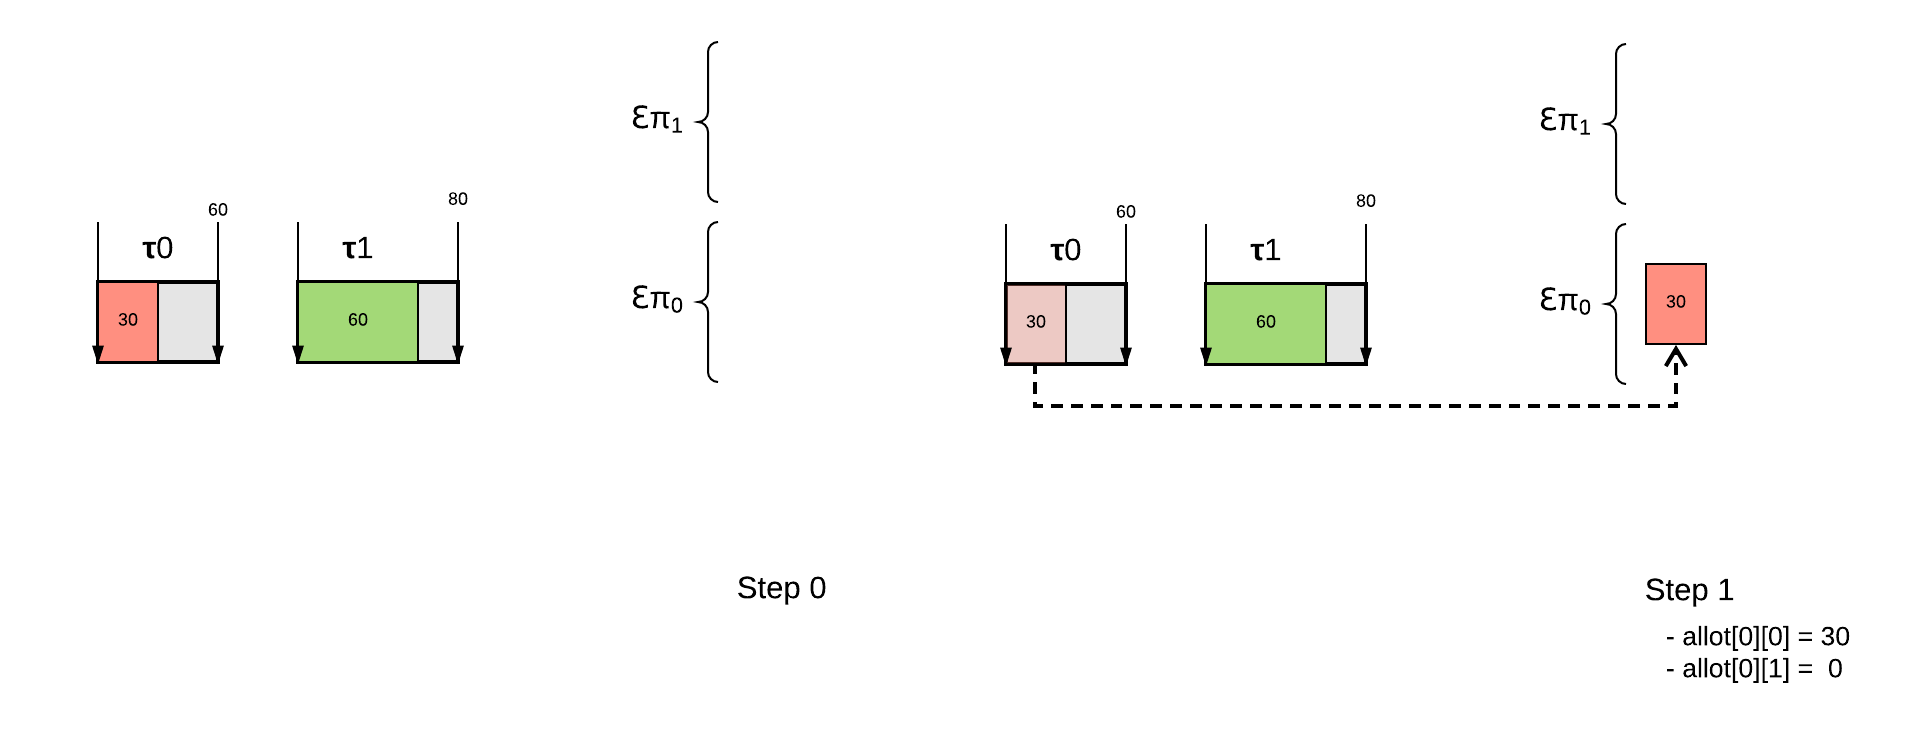
\includegraphics[scale=1]{img/uedf/uedf12}
		\caption{étapes 0 et 1}
	\end{figure}
	\begin{figure}[H]
		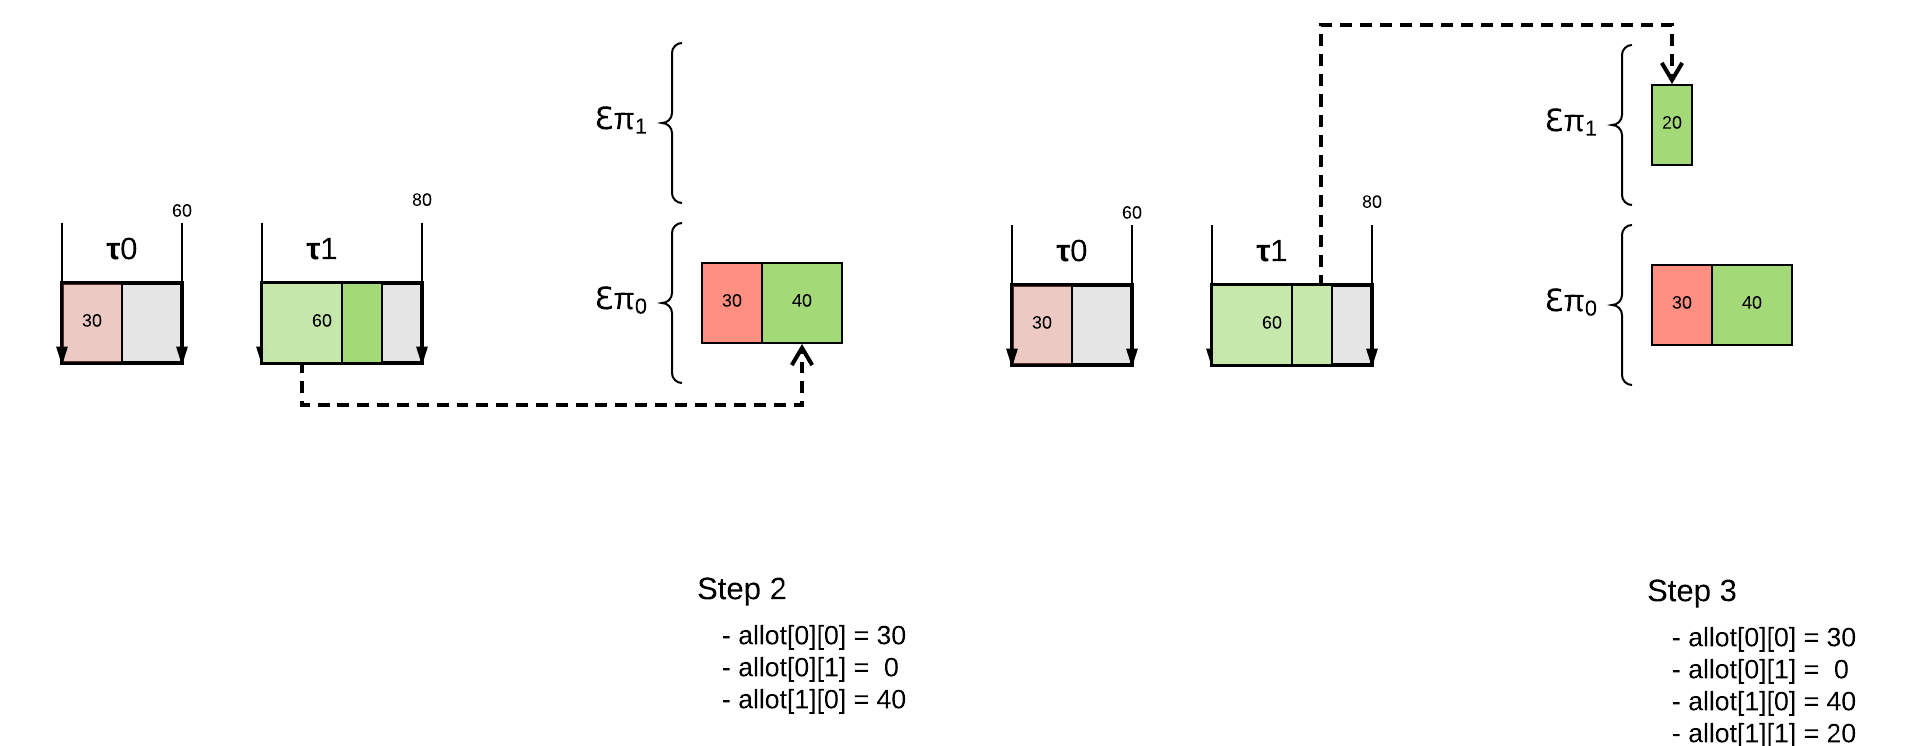
\includegraphics[scale=1]{img/uedf/uedf34}
		\caption{étapes 2 et 3}
	\end{figure}
	\subsubsection{Eligible}
	À ce stade, aucune décision d'ordonnancement n'est encore prise, mais des ensembles de tâches (\textit{Eligible}, 
	noté $\epsilon$ dans la suite) sont créés sous forme de listes. Chaque liste \textit{Eligible} définit 
	les seules tâches que les processeurs associés peuvent exécuter (en cela, cette phase d'\textbf{UEDF} peut 
	être considérée comme une phase de partitionnement) durant l'exécution à venir.\newline
	
	Notons que les calculs fournis par l'algorithme permettent en théorie de \og{}remplir\fg{} 
	la charge d'un processeur à 100\% d'utilisation avant de passer au suivant. Concrètement, 
	cela signifie que si la première tâche a une utilisation de moins de 100\%, elle sera suivie par 
	au moins une partie d'une autre.\newline
	
	Les valeurs d'$Allot$ ne doivent pas être considérées comme le temps d'exécution qui sera réellement 
	exécuté sur le processeur. Il faut garder à l'esprit qu'à chaque relâchement de travail, 
	$Allot$ sera recalculé. 

	\subsubsection{Prise de décision}
	La phase de décision de l'ordonnancement se déroule lors de la phase suivante.
	\textbf{UEDF} s'inspire pour finir de \textbf{EDF-Delay}. 
	Cet algorithme est très simple :
	\begin{itemize}
		\setlength\itemsep{0.1em}
		\item Une tâche $\tau_i \in \epsilon_j, j \in m$ est attribuée à un processeur $\pi_j$ si aucun autre processeur d'index plus bas n'est en train de l'exécuter
		\item $\tau_i$ s'exécute sur le processeur $\pi_j$ tant qu'$allot_{ij} > 0$
	\end{itemize}


	\subsubsection{Déroulement}	
	L'algorithme \hyperref[algouedf]{$Compute Allot$ [\ref*{algouedf}]} est à effectuer à chaque relâchement de tâche. La valeur $Allot_{ij}$ 
	doit être mise à jour à chaque prise de décision. Une décision est attendue pour chacun des événements suivants :
	\begin{itemize}
		\setlength\itemsep{0.1em}
		\item Une instance de tâche (travail) a été relâchée\\
		 $\sum_{i \in A(t)}\sum_{1}^{m}allot_{ij} = WCET$
		\item Le temps alloué sur un processeur a été exécuté, dans ce cas\\ $\exists i \in A(t), \exists j \in m : allot_{ij} = 0$
		\item Un travail est terminé complètement : \\
		$\sum_{i \in A(t)}\sum_{1}^{m}allot_{ij} = 0$.
	\end{itemize}
	
	On peut voir en théorie l'ordonnancement de trois tâches en annexe, afin de mieux comprendre le déroulement d'une exécution.
	À titre de remarque, le travail d'illustration d'une exécution nous semble 
	important pour procéder à une implémentation, sinon le risque est d'omettre le développement 
	d'outils indispensables au bon déroulement de l'exécution. L'algorithme n'est pas trivial à mettre en œuvre.
	\todo{gantt chart avec exemple 30;60, 60; 80, 60;80}
	\newline
	
	Nous pouvons déjà formuler ici une nuance par rapport à la théorie et les attentes que l'on peut en avoir 
	en pratique : 
	nous savons dès le départ que l'algorithme \textbf{UEDF} est assez gourmand en calcul puisque chaque relâchement de 
	tâche va provoquer l'exécution de l'algorithme $Compute Allot$, or, le calcul de cette valeur 
	implique un parcours de toutes les tâches ordonnées, pour chaque processeur. 
	Outre qu'il est nécessaire de gérer une structure de données efficace, nous pouvons 
	déjà considérer que le tri de la structure sera d'un coût non négligeable lors de l'exécution. \newline
	
	Par ailleurs, le calcul même de $Compute Allot$ implique lui aussi une certaine complexité.
	Ainsi :
	\begin{itemize}
		\setlength\itemsep{0.1em}
		\item soit $m$ le nombre de processeurs
		\item soit $n$ le nombre de tâches actives [\ref*{tacheactive}] du système
		\item $Compute Allot \in O(m\times n)$
	\end{itemize}

	Et pour finir, régulièrement, la valeur $allot_{ij} \forall i \in TaskSet, \forall j \in m$ doit être mise 
	à jour, dont la complexité est donc :
	\begin{itemize}
		\setlength\itemsep{0.1em}
			\item soit $m$ le nombre de processeurs
			\item soit $n$ le nombre de tâches actives [\ref*{tacheactive}] du système
			\item $update Allot \in O(m\times n)$
	\end{itemize}

	Nous pouvons attendre un surcoût important sur cette base. Une hypothèse étant que ce surcoût 
	augmente avec le nombre de tâches, mais aussi avec le nombre de cœurs. Un même système pourrait avoir plus 
	de surcoût avec plus de cœurs. Cela pourra être vérifié dans les expérimentations.

	
	\subsection{Comparaison avec Global-EDF}
	
	Nous avons choisi de comparer \textbf{UEDF} à \textbf{Global-EDF} [\ref*{GlobalEDF}]. 
	La raison de ce choix est simple : 
	cet algorithme est implémenté sur le RTOS HIPPEROS et il est global, comme 
	l'indique son nom. 
	Les autres ordonnanceurs disponibles sur HIPPEROS sont pour la plupart partitionnés.
 
	Aussi les tests effectués sur \textbf{UEDF} seront également faits en utilisant \textbf{Global-EDF} pour 
	élément de comparaison.\newline
	
	Ces deux algorithmes ont toutefois de grandes différences. \textbf{Global-EDF}
	ne permet pas - même théoriquement  d'atteindre l'optimalité. Ceci s'explique par le fait que 
	\textbf{Global-ED}F peut être considéré comme \og{}vertical\fg{} là où \textbf{UEDF} serait \og{}horizontal\fg{}. 
	Mais une grande différence entre les deux algorithmes est que \textbf{Global-EDF} n'est optimal, 
	en théorie, contrairement à \textbf{UEDF}.
	
	\subsubsection{Fonctionnement de Global EDF}
	
	L'algorithme est relativement simple, et pour les besoins de la comparaison, nous résumons 
	ici son fonctionnement.\\
	À un moment \textit{t}, l'ordonnanceur prend sa décision de cette façon :
	si un processeur est libre, il se voit attribué le travail de priorité supérieure parmi 
	tous les travaux actifs et pas encore attribués. Cela permet d'avoir un algorithme peu gourmand.
	
	\begin{algorithm}
	\caption{Global-EDF}
	\begin{algorithmic}
		\REQUIRE $JobList(t)$ ordonné par échéances
		\FORALL{ $j \in m $}
			\item $decision \leftarrow pop(JobList(t))$
		\ENDFOR
	\end{algorithmic}
\end{algorithm}	
	
	L'algorithme permet de prendre une décision au moment \textit{t} en ne considérant 
	que les travaux à exécuter par ordre de priorité et les processeurs disponibles.
	
	Si l'on reprend l'exemple illustré précédemment, la décision sera prise de cette façon :
	
	\begin{figure}[H]
		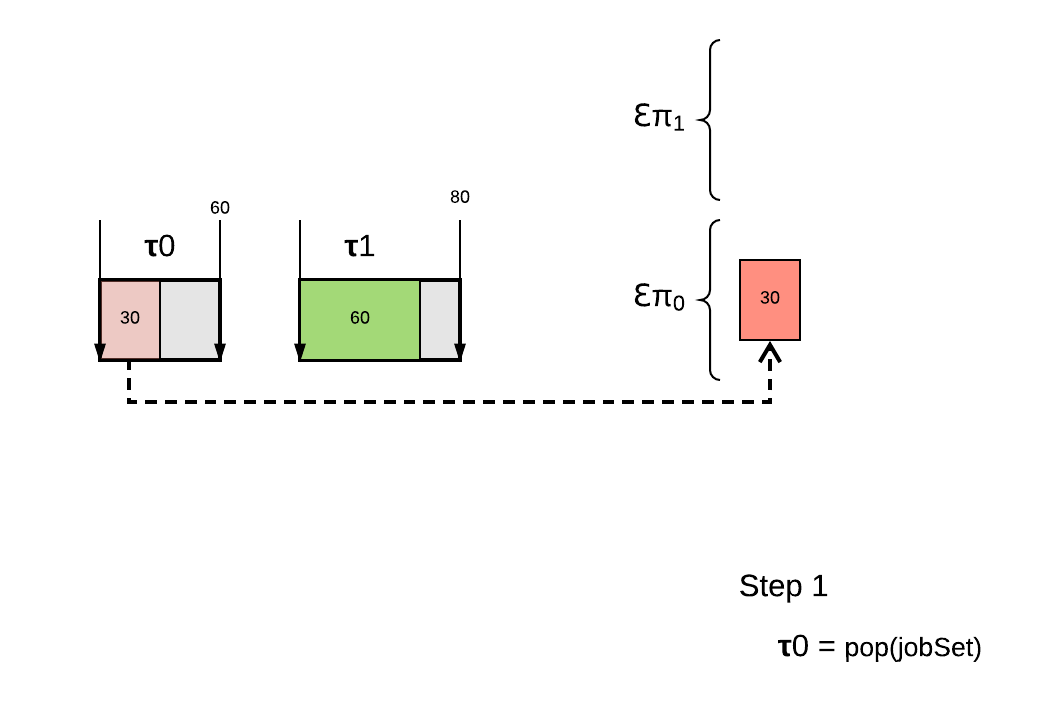
\includegraphics[scale=0.5]{img/gedf/gedf}
		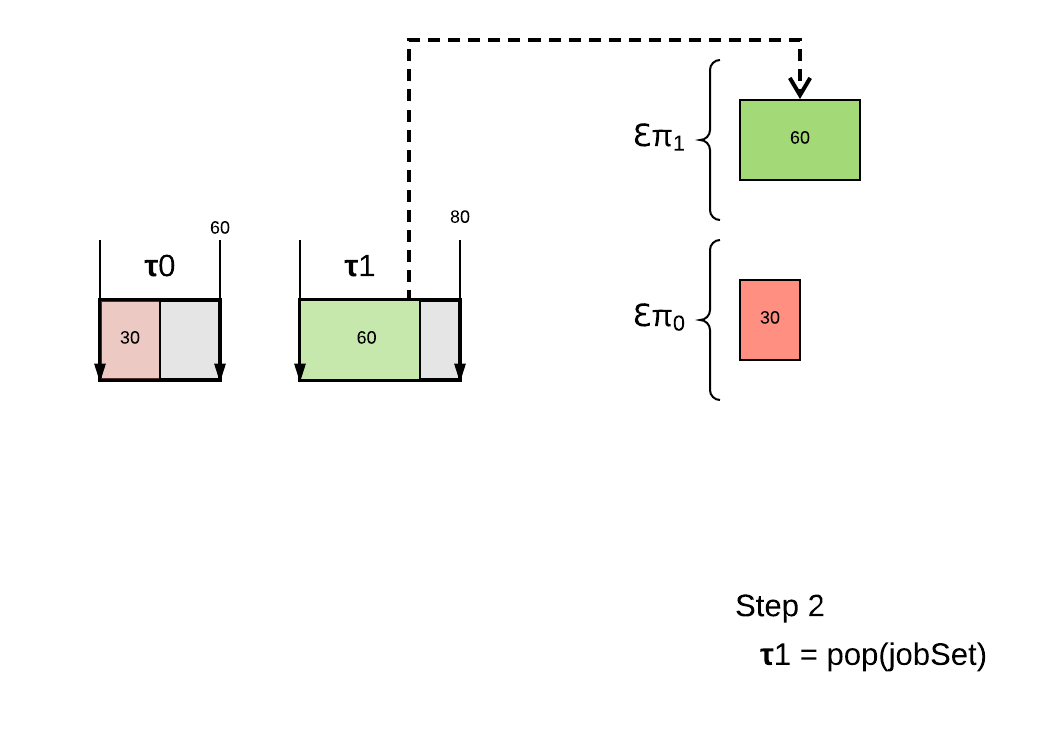
\includegraphics[scale=0.5]{img/gedf/gedf2}
		\caption{Global EDF}
	\end{figure}
	 
	On peut facilement voir que cela peut entraîner de \og{}mauvais choix\fg{}. 
	En changeant l'exemple précédent, et en prenant un exemple avec 3 travaux, 
	on n'obtiendra pas du tout le même ordonnancement dans les deux algorithmes, 
	et celui-ci mettra en échec \textbf{Global-EDF} quasiment immédiatement.\newline
	
	Prenons un ensemble de trois tâches comme suit :

	\begin{enumerate}
		\setlength\itemsep{0.1em}
		\item $\tau_1 : \{o:0; w:40; d=p:60;\}$
		\item $\tau_2 : \{o:0; w:40; d=p:60;\}$
		\item $\tau_3 : \{o:0; w:40; d=p:60;\}$
	\end{enumerate}
	
	\todo{insérer schema ici}
	
	Malgré ce point, \textbf{Global-EDF} est \og{}efficace\fg{} en terme de calculs.
	Le point le plus complexe concerne la structure de données qui conserve les 
	tâches courantes. Une bonne idée est d'utiliser un Heap [\ref*{heap}] qui 
	va permettre de fournir toujours en tête le travail de priorité supérieure.
	Pour s'assurer de la faisabilité de l'ensemble de tâches, 
	il faudra tester l'ordonnancement suffisamment longtemps (hyper-période).\newline

		
\section{HIPPEROS}
	\customhighlight{HIPPEROS} (\textbf{HI}gh \textbf{P}erformance \textbf{P}arallel \textbf{E}mbedded \textbf{R}eal-time \textbf{O}perating \textbf{S}ystems)
	est un \customhighlight{RTOS} (Real-Time Operating System) développé depuis plusieurs années par une spinoff de l'ULB.
	Il bénéficie des connaissances apportées par le monde de la recherche dans 
	le domaine des systèmes critiques avec multic\oe{}urs. Une de ses particularités 
	est sa modularité, qui permet d'adapter ses possibilités en fonction du système 
	lors de la compilation de l'OS, ainsi peut-on différencier principalement 
	deux installations en fonction des particularités. 
	
	\customhighlight{HIPPEROS} est un candidat idéal pour l'implémentation d'un ordonnanceur 
	global. Il a cependant un fonctionnement propre qui pourra rendre l'implémentation 
	plus ou moins facile. Par exemple, HIPPEROS, à l'inverse de \textit{Linux}, a un ordonnanceur 
	asymétrique (un processeur est \textit{Master}, et les autres sont \textit{Slaves}).
	En d'autres termes, l'ordonnancement est calculé uniquement sur l'un des processeurs, 
	qui sera désigné au moment de la compilation. 
	Cela simplifie l'implémentation, puisque l'on ne doit pas s'occuper de savoir quel processeur est 
	actuellement en train d'effectuer l'algorithme d'ordonnancement.\newline
	En résumé, une nouvelle implémentation sur un OS différent 
	peut elle-aussi apporter à la connaissance générale des détails importants.\newline
	
	Notons qu'HIPPEROS est un RTOS privé, avec les conséquences logistiques que l'on peut 
	imaginer : la documentation est privée également, et pour comprendre le kernel, la 
	seule ressource est l'équipe de développeurs qui l'a créé. 
	
		
\section{Attentes}

	Des présentations des différents acteurs qui ont été faites dans les parties précédentes, à savoir :
	\begin{enumerate}
		\setlength\itemsep{0.1em}
		\item UEDF
		\item Global-EDF
		\item HIPPEROS
	\end{enumerate}
	Nous pouvons déjà formuler certaines hypothèses que nous aimerions vérifier dans ce travail. \newline
	
	\begin{itemize}
		\item Vérifier que l'algorithme ne comporte rien qui empêche son implémentation dans 
		HIPPEROS
		\item Mesurer les surcoûts liés à l'algorithme \textbf{UEDF}, car il n'est pas 
		évident qu'il soit possible de l'utiliser en pratique.
		\item Vérifier également si l'on observe bien en pratique que \textbf{Global-EDF} ne 
		peut pas ordonnancer certains systèmes là où \textbf{UEDF} le peut.
		En effet, il est possible que ce résultat soit modifié ou largement à nuancer en 
		fonction de certains paramètres, comme le WCET, dont nous reparlerons.
		\item Comparer le nombre de migrations/préemptions obtenues pour un même système, ordonnancé 
		par l'un ou l'autre des algorithmes, on peut s'attendre à ce qu'\textbf{UEDF} soit performant à ce niveau.
	\end{itemize}


	
\chapter{Implémentation}

\vspace*{\fill} \epigraph{\itshape Every good idea will be discovered twice. Once by a logician, and once by a computer scientist.}{\vspace*{12pt} Philip Wadler}
\vfill\clearpage


	
	Une partie du travail consiste à évaluer si \textbf{UEDF} est implémentable. 
	La réponse est oui, car nous avons une implémentation fonctionnelle et fidèle à la description 
	théorique de l'algorithme. \newline
	
	Néanmoins, il nous semble utile d'exposer nos choix, afin de permettre à de nouveaux candidats 
	à l'exercice de profiter de nos essais/erreurs. Également, cela permet de comprendre les 
	résultats qui suivent, et de proposer des améliorations pour le futur.\newline
	
	Dans la partie qui suit, nous détaillons l'implémentation faite dans \textbf{HIPPEROS} pour ce travail, 
	et pour ce faire, nous devons aborder des points de détails liés à l'algorithme, 
	à l'implémentation, ou même à \textbf{HIPPEROS}.

	\subsubsection{Données temporelles}
	
		Dans \textbf{HIPPEROS}, il existe plusieurs ordonnanceurs déjà implémentés. 
		Ils ont leur fonctionnement propre, et de façon générale, sont assez différents d'\textbf{UEDF} par 
		rapport aux variables auxquelles ils accèdent. 
		\textbf{UEDF} a besoin de l'\textit{utilisation} d'une tâche dans certains de ses calculs. Or, l'\textit{utilisation} 
		est une fraction. Nous souhaitons éviter la représentation à virgule flottante 
		pour gérer ces fractions, et par conséquent, cela nécessite un décalage des valeurs.\newline
		 
		Se pose alors la question du décalage à appliquer afin d'occuper une place raisonnable en ayant 
		le moins de pertes possibles.  
		La réponse à apporter diverge en fonction de plusieurs facteurs :
		appelons le décalage $SHIFT$.
		\begin{itemize}
			\setlength\itemsep{0.1em}
			\item Pour rappel, l'\textit{utilisation} est définie de la sorte : $U(i) \defeq \frac{C_i}{T_i}$. 
			%\todo{def mots, ajouter utilisation, deadline, signalétique}
			En pratique, c'est le \textit{WCET} et la période de la tâche que l'on utilise pour calculer cette fraction : 
			$\frac{WCET}{T_i}$.
			HIPPEROS stocke les valeurs temporelles $wcet$ et $period$ en entiers non signés sur $64$ bits.
			
			\item Le décalage $SHIFT$ doit être choisi en fonction du rang des valeurs que l'on peut obtenir.
			Nous pouvons négliger les tâches de moins de $1 \%$ d'utilisation pour conserver un rang de $1$ à $100\%$.
			Concrètement, nous pourrons avoir les valeurs de $\frac{SHIFT}{100}$ à $SHIFT$.
			\item En théorie, le nombre de processeurs est libre. En pratique, 
			notre matériel ne dépassera pas les 4 cœurs, aussi aurons-nous une utilisation maximale de $400\%$.
			Quand bien même nous irions plus loin, nous ne dépasserions pas les 8 cœurs pour des raisons 
			matérielles, donc 800\% : $SHIFT \times 8$.
			\item En reprenant l'algorithme en section \ref{algouedf}, 
			l'\textit{utilisation} sert à multiplier la différence entre deux échéances de travaux différents.
			Cette valeur est libre, et on peut l'imaginer grande dans certains cas. 
			Admettons qu'une tâche ait une échéance de $8.000.000 \mu s$, et une autre du double, comme cela 
			peut tout à fait se croiser dans un cas pratique, on aura une différence de $8.000.000$ à multiplier
			par cette proportion. 
			La valeur limite d'un entier de $64$ bits étant $2^{64} - 1$ ($18.446.744.073.709.551.615$), nous pouvons estimer que la marge 
			est grande et nous laisse libre de choisir un décalage grand.
		\end{itemize}
		Pour ces raisons, dans notre implémentation, nous avons estimé que décaler les valeurs de $1000$ était un bon compromis.
		Par exemple, pour une tâche qui serait définie comme suit : $\tau_1 = \{w:1; d=p : 3\}$, 
		l'\textit{utilisation} sera $\frac{1000}{5000} = 200$.
		Une \textit{utilisation} de $1\%$ est stockée dans l'implémentation d'\textbf{UEDF} comme une utilisation de 
		$10$, tandis qu'une de $100\%$ vaudra $1000$. Ce décalage sert dans tout l'\hyperref[algouedf]{algorithme décrit en section [\ref*{algouedf}]}.
		Aussi, toutes les variables seront décalées d'autant, comme l'index du processeur, afin d'avoir un calcul cohérent. 
		Toutefois, le nombre d'unités de temps $allot$ 
		n'est lui-même pas décalé, afin de contenir le bon nombre d'unités de temps à exécuter pour la suite.		
		
	\subsection{Structures de données}
		Dans ses nombreux calculs, \textbf{UEDF} fait appel à un certain nombre de données concernant les tâches ou les travaux.
		Mais l'ordonnanceur a également besoin d'accéder à des variables qui lui sont 
		spécifiques à divers moments de l'exécution. 
		En outre, il doit également conserver les travaux n'ayant pas atteint leur échéance, 
		car, entre deux relâchements de tâche, un travail $i$ peut se terminer ou être préempté, 
		il continue cependant de \og{}peser\fg{} dans l'ordonnancement au temps $t$ tant que $t < d_i(t)$.
		\newline
				
		\paragraph{Allot}
		Les valeurs du tableau multidimensionnel $Allot$ sont primordiales et doivent être conservées durant l'exécution.
		Elles permettent de décider si une tâche doit être exécutée ou non.
		Elles devront être actualisées à chaque événement.
		Ainsi, on doit conserver un tableau à deux dimensions $Allot$, qui contient des données 
		temporelles (entiers non signés de $64$ bits). 
		Cette structure est de taille $m \times n$ en théorie. 
		En pratique, dans \textbf{HIPPEROS}, $m$ et $n$ sont des valeurs prédéfinies 
		dans chaque version. Le nombre de tâches peut être à ce jour $32$, $128$ ou $1024$.
		Il ne nous a pas semblé utile de changer cela. Nos tests ont tous pour configuration 
		un nombre de tâche maximum de 32. 
		\newline
		
		L'algorithme de calcul du tableau $Allot$ (\hyperref[algouedf]{$Compute Allot$[\ref*{algouedf}]}) attribue les travaux
		aux processeurs par ordre ascendant d'index. Notre implémentation s'est adaptée à \textbf{HIPPEROS}, car c'est le 
		cœur $0$ le \textit{Master}, qui exécute l'algorithme d'ordonnancement. Par conséquent, 
		nous avons inversé l'ordre, pour que le cœur $0$ soit le dernier \og{}rempli\fg{} par l'algorithme -- 
		ce -- dans le but d'éviter que les surcoûts rendent des ensembles non faisables. Ainsi, 
		pour $4$ cœurs, une exécution jusqu'à $300\%$ d'\textit{utilisation} laissera le cœur $0$ 
		uniquement occupé à gérer l'ordonnancement.
		
		\paragraph{Liste triée de tâches}
		Il est nécessaire de maintenir à jour un ensemble trié de tâches, pour le 
		calcul d'$Allot$. Pour cette structure, notre choix a beaucoup évolué au cours du temps. 
		La première idée était le besoin de parcourir cette liste dans l'ordre, plusieurs fois, 
		d'y ajouter et d'en retirer des éléments. A priori, pour ces raisons, le \textit{Heap} ne 
		correspond pas bien à nos besoins, aussi avons-nous utilisé une liste liée en 
		premier lieu. Néanmoins, les mauvaises performances de la liste liée 
		nous ont amené à reconsidérer ce choix, d'autant plus que les parcours de listes étaient nombreux. 
		À l'heure actuelle, notre implémentation construit un \textit{Heap} avant le recalcul d'$Allot$.
		Ce \textit{Heap} est copié chaque fois avant d'en faire le parcours, dans les diverses parties du code.
		En pratique, lorsque des travaux sont relâchés, nous parcourons à l'heure actuelle 3 fois ce \textit{Heap}, 
		chaque fois copié au préalable. 
		Ce choix a fait diminuer drastiquement le surcoût par rapport au choix de la liste liée, 
		néanmoins reste perfectible.
		%\todo{ajouter citation qui dit qu'il faut pas optimiser avant d'avoir bien implémenté, knuth}
		Par exemple, il est tout à fait imaginable de ne pas reconstruire le \textit{Heap} à chaque fois qu'il faut 
		calculer $Allot$, il faudrait maintenir une structure persistante, et mieux gérer les activations ou suppressions. 
		C'est une amélioration simple qui n'a pas encore été faite, et pourrait réduire légèrement les surcoûts.
		%\todo{ptete essayer avant la remise, ça pourrait se faire facilement je pense.} 
		\newline
		
		\paragraph{Liste d'états}
		Une première chose à laquelle il faut être attentif est de rendre possible les accès 
		aux données, par exemple en conservant des tableaux de références, afin de minimiser les temps 
		d'accès. Cela nécessite de faire un choix : on optimise le temps d'accès en conservant plus de données. 
		L'ordonnancement en cours est ainsi doublement référencé : 
		\begin{itemize}
			\setlength\itemsep{0.1em}
			\item $Job\_id \leftarrow coreToSchedule_{core}$ permet d'obtenir le travail en cours d'exécution sur le processeur $core \in m$
			\item $core \leftarrow scheduledToCore_{job\_id}$ permet d'obtenir le processeur qui exécute le travail $job\_id \in n$.
		\end{itemize}

		Nous devons également conserver les divers états d'un travail. En effet, rappelons que dans \textbf{UEDF}, 
		un travail est considéré comme \textit{actif} tant qu'il n'a pas rencontré son échéance -- et ce, 
		même s'il est \textit{terminé}. Nous conservons donc un tableau d'états permettant 
		d'accéder facilement à cette information.
		De même, nous devons différencier l'état \textit{bloqué} d'un travail \textit{terminé}, ce qui n'est pas le cas 
		dans les autres ordonnanceurs implémentés dans \textbf{HIPPEROS}. Par exemple, dans \textbf{Global-EDF}, si un travail 
		attend une ressource, la tâche correspondante au travail bloqué sera purement et simplement retiré de la liste de tâches actives, 
		et lorsqu'elle sera réactivée, elle sera réintroduite dans cette liste. Ce comportement n'est pas possible dans \textbf{UEDF}, 
		qui \og{}réserve\fg{} du temps, et \og{}prévoit\fg{} un ordonnancement. Si le travail sort, et est simplement 
		réintroduit, cela provoquerait un nouveau calcul d'$Allot$, basé sur le $WCET$, et pas le temps restant d'exécution.
		
	\section{WCET, et Temps d'exécution}
		
		Les autres ordonnanceurs implémentés dans \textbf{HIPPEROS} n'utilisent pas les données concernant le temps 
		d'exécution de la tâche dans leur prise de décision. 
		Pour \textbf{UEDF}, nous avons besoin d'un accès efficace et correctement mis à jour à ces données. 
		Typiquement, le \textbf{Temps d'exécution restant}(\textbf{RET}) est utilisé pour le calcul et la mise à jour 
		d'\textbf{Allot}.\newline
		
		En pratique, \textbf{HIPPEROS} met à jour le temps exécuté d'un travail lors d'un événement qui le concerne. 
		Ainsi, si un travail est effectué, on note le moment où le travail a été dispatché.
		Au temps \textit{t}, si l'on veut savoir combien de temps a déjà été exécuté, 
		s'il n'a pas croisé d'événement, il faudra calculer ce temps dans \textbf{UEDF} 
		car \textbf{HIPPEROS} n'aura pas encore mis à jour cette donnée.\newline
		Si en terme de temps d'accès, cette requête n'est pas très compliquée, il n'en demeure pas moins 
		que le résultat sera un peu approximatif, puisque l'ordonnanceur n'arrête pas l'exécution des tâches pendant 
		son exécution. Cela ne change pas fondamentalement le calcul car cela change très faiblement les valeurs, 
		mais cela constitue une adaptation de la théorie en pratique.\newline

	\section{Modèle VS réel}
	
		Dans un modèle, l'exécution s'arrête, l'algorithme d'ordonnancement est effectué, 
		puis les travaux sont dispatchés et l'exécution reprend.
		Le surcoût peut être totalement ignoré.
		\newline
		
		L'ordonnanceur ne fait pas partie de l'ensemble des tâches du système. Cependant, il est exécuté 
		sur un des processeurs, et occupe une charge non nulle de temps. Outre que cela fausse les calculs 
		liés à la charge possible (concrètement, les 100\% d'utilisation libres sur le cœur qui exécute 
		les actions de l'ordonnanceur ne sont plus 100\% mais sont amputés du surcoût), 
		cela créé un décalage entre les valeurs calculées au moment $t$ et le moment réel de l'exécution.
		Il faudra adapter les WCET des tâches en fonction de cela, ce qui implique 
		une partie du travail qui consiste à évaluer le surcoûts, ainsi que de proposer une 
		façon de déterminer les WCET de tâches.\newline
		
	\section{Événements et calcul de l'ordonnancement}

		Dans HIPPEROS, voici une exécution typique :
		\begin{itemize}
			\setlength\itemsep{0.1em}
			\item Des tâches sont activées
			\item Le \textit{dispatcher} demande à l'ordonnanceur de calculer l'ordonnancement
			\item Le \textit{dispatcher} prend les décisions de l'ordonnanceur et effectue les changements 
			s'il y a lieu (dispatcher une tâche, en préempter une autre, etc.)
			\item Des événements viennent réveiller le \textit{dispatcher}, comme la fin, 
			la préemption, ou le relâchement d'un travail. Entre deux événements, l'exécution 
			de chacun des travaux sur les processeurs a lieu sans interruption.
		\end{itemize}
		
		Concrètement, c'est une fonction \textit{compute\_schedule} qui est appelée, sans 
		que l'on sache forcément quel événement a provoqué son appel. \newline
		
		Or, dans \textbf{UEDF}, il est nécessaire de différencier les moments où un travail a été relâché 
		d'un autre, où l'on ne devra pas recalculer $Allot$. Il suffit dès lors d'activer un 
		booléen indiquant qu'un nouveau travail a été relâché. Si ce booléen est vrai, 
		l'algorithme calcule totalement $Allot$, dans le cas contraire, il ne fait que mettre ses valeurs à 
		jour, avant de prendre dans les deux cas une décision.\newline
	
	\section{Domaine système}
	Dans le monde des systèmes embarqués, la norme \textbf{P}ortable \textbf{O}perating \textbf{S}ystem \textbf{I}nterface (\hyperref{http://www-sop.inria.fr/chir/personnel/arias/NArgimoge/Document/node19.html}{POSIX}{POSIX}{POSIX})	
	est une spécification des fonctions de base d'un système d'exploitation. Afin de permettre la portabilité des programmes, 
	cette norme garantit des propriétés quant à l'implémentation de certaines fonctions. \newline	
	
	L'ordonnanceur est chargé d'ordonnancer les tâches selon leurs priorités. 
	La norme \textbf{POSIX} définit des niveaux pour les threads : \textit{local}, et \textit{System}. 
	Mais en pratique, \textbf{Linux} n'utilise pas cela, tous les \textit{Threads} sont 
	de niveaux \textit{System}, et il ne gère pas de \textit{Process} comme ensemble de \textit{Threads}.\newline

	Une variante importante ressort ici : \textbf{HIPPEROS} gère des \textit{Process}, 
	qui sont des ensembles de \textit{Threads}. L'ordonnanceur gère des \textit{Process}, qui ont un ou plusieurs \textit{Threads}, 
	et les priorités pour chacun d'eux sont locales.
	C'est dans le but de gérer des exceptions et interruptions au niveau utilisateur qu'\textbf{HIPPEROS } a implémenté 
	des niveaux différents de domaines. S'il est du domaine \textit{system}, un \textit{Process }est de priorité supérieure, quoi que décide 
	l'ordonnanceur. Cela s'explique de cette manière :\newline

	Concrètement, on imagine une sonde qui envoie très rarement des données. On ne réserve 
	pas de temps d'exécution régulier pour effectuer cette écoute, 
	on vérifie simplement régulièrement qu'elle a des données à traiter, et si c'est le cas, on les traite.\newline
	
	C'est un cas d'utilisation du domaine \textit{System} : garantir que les données seront traitées vite, dès qu'elles arrivent, 
	sans attribuer une tâche pour le faire régulièrement.\newline
	
	Notre solution pour gérer cette situation avec \textbf{UEDF} est simplement de faire passer en priorité 
	la tâche du domaine \textit{System} s'il y en a une, sans la comptabiliser dans \textbf{UEDF}. 
	Cela pourrait invalider potentiellement un système, puisqu'on peut en théorie 
	exécuter une proportion de temps qui n'a pas été comptabilisée dans l'ordonnanceur. 
	Nous conseillons dans ce cas d'adapter d'autant le WCET des tâches.
	
	
\chapter{Méthodologie}
\vspace{100pt}
\begin{center}
	\includegraphics[scale=0.5]{img/good_code}
	
	\textit{xkcd}
\end{center}
\vfill\clearpage

	\section{Choix de l'ordonnanceur}

	\subsection{Pourquoi UEDF}
	
	L'état de l'art nous a montré un vaste choix d'algorithmes intéressants pour différentes 
	raisons et n'étant pas encore implémentés. La première étape du travail consiste donc 
	à départager ces algorithmes pour arrêter notre choix sur l'un d'entre eux.
	
	Le choix le plus rationnel vis à vis des objectifs devrait se faire en fonction des 
	promesses théoriques de performance et de stabilité. 
	En effet, pour faire avancer la connaissance et permettre d'augmenter la confiance des utilisateurs 
	potentiels, il est judicieux de choisir un algorithme dont on attend au moins ceci :
	\begin{itemize}
		\item Un algorithme global qui minimise le nombre de migrations
		\item L'ordonnanceur est en ligne, optimal pour la classe périodique
		\item Il n'a pas bénéficié d'une implémentation sur un \textbf{RTOS}
		\item Il promet des performances intéressantes
	\end{itemize}
	
	Le premier choix a été \textbf{RUN}, puis finalement, son descendant, \textbf{QPS}. Ces choix étant guidés 
	sur leur intérêt en tant qu'ordonnanceurs en tant que tels.
	Toutefois, les papiers disponibles étaient assez théoriques. En outre, nous n'avons pas 
	trouvé d'implémentation ou de simulation malgré nos recherches.
	Finalement, nous n'avons pas réussi à entrer en contact avec les créateurs de ces algorithmes. 
	
	Aussi nos questions restaient sans réponses, or, elles auraient pu permettre une implémentation 
	malgré les obstacles précédemment cités.\newline
	
	Ceci est peut-être une première remarque à faire à propos de la possibilité d'implémenter 
	un ordonnanceur : avoir un contact possible avec une personne à son origine -- voire qui a déjà 
	réussi une implémentation -- rend le travail bien plus simple, en fonction des 
	explications disponibles à l'origine.\newline
	
	
	Finalement, c'est donc un argument quant à la communication (clarté, possibilité de poser des questions) 
	qui a fixé le choix. Par conséquent, c'est \textbf{UEDF} qui a été sélectionné, car 
	non seulement il respectait 
	les promesses énoncées auparavant, mais aussi, en plus d'être très bien documenté, 
	 nous pouvions poser nos questions directement à l'un de ses créateurs. Néanmoins, ses paramètres sont moins idéaux, 
	et nous avons revu nos attentes quant à l'efficacité à la baisse. Cela n'a en rien 
	modifié l'objet scientifique, à savoir le regard critique et la proposition d'améliorations 
	afin de stimuler et faciliter des implémentations futures.\newline
	
	
	Nous avons déjà présenté précédemment \textbf{UEDF}, de façon globale et succincte. 
	Dans cette partie, nous allons un peu plus en profondeur.
	
	
	\subsection{Présentation UEDF}
	\textbf{UEDF} est un ordonnanceur qui comporte plusieurs intérêts pour une implémentation.
	Tout d'abord, il est principalement \textit{en ligne}\todo{verif glossaire}, ce qui n'est pas le cas de 
	la plupart des ordonnanceurs utilisés dans l'industrie.
	Ensuite, il est global.\todo{include lien vers glossaire} Or, la plupart des ordonnanceurs 
	globaux connus et implémentés ne sont pas optimaux (pour la classe périodique), pour la
	raison exposée au préalable dans ce travail : il est nécessaire d'avoir de la clairvoyance, 
	c'est à dire une connaissance relative du futur.\newline
	
	Globalement, \textbf{UEDF} va réserver du temps sur les processeurs pour toutes les tâches actives.
	Rappelons que pour \textbf{UEDF}, une tâche est considérée comme active entre le moment où la tâche 
	a relâché un travail, et l'échéance, même si l'exécution de cette tâche a déjà été effectuée.
	Pour ce faire, un calcul va permettre de réserver du temps sur chaque processeur.
	
	\textbf{UEDF} fait face à ce problème en ayant un traitement non pas vertical, mais horizontal
	de l'ordonnancement des tâches.	

	\todo{inclure image de slice}
	À ce stade, aucune décision n'est prise, mais on dispose d'un ensemble de sous-systèmes qui peuvent 
	être exécutés sur les processeurs à condition qu'$Allot_{ij} > 0$ où $i$ est une tâche, 
	et $j$ le processeur.
	

		\subsubsection{Fonctionnement très général de Global EDF}
		Afin de montrer la particularité d'\textbf{UEDF}, nous commençons par rappeler le fonctionnement 
		d'un ordonnanceur bien connu et que l'on peut considérer comme "vertical" : \textbf{Global EDF}. \todo{link état de l'art}
		
		L'algorithme est extrêmement simple, et pour les besoins de la comparaison, nous rappelons 
		ici son fonctionnement de façon très résumée.\\
		À un moment \textit{t}, l'ordonnanceur prend sa décision de cette façon :
		si un processeur est libre, il se voit attribué le travail de priorité supérieure parmi 
		tous les travaux actifs. Cela permet d'avoir un algorithme extrêmement simple :\newline
		
		
		On conserve une structure de données 
		ordonnée, comme un \textbf{Heap} \todo{glossaire} qui contient tous les travaux
		devant être exécutés. À chaque fois que l'ordonnanceur doit prendre 
		une décision, il lui suffit de prendre le travail de priorité supérieure et 
		de l'exécuter sur le processeur libre.
		
		L'algorithme ne calcule rien à propos de l'avenir, sa décision au moment \textit{t}
		n'est prise qu'en considérant les jobs à exécuter et la liberté d'un 
		processeur. Il se peut qu'un autre ordonnancement plus efficace 
		réussisse à ordonnancer un système que \textbf{Global EDF} ne puisse pas résoudre...
		Cela rend tout de même l'ordonnanceur "efficace" en terme de calculs, 
		puisqu'il comporte un Heap, de complexité $O(n\log n)$, qui sera mis à jour 
		à chaque changement d'état du job (relâché -> inséré, 
		exécuté -> retiré du Heap).
		
		En revanche, ce fonctionnement ne permet pas à cet ordonnanceur d'atteindre 
		l'optimalité pour la classe de systèmes périodiques, comme on peut le voir 
		avec cet exemple :
		\todo{montrer un exemple qui rende Global EDF non efficace pour un job}

		\subsubsection{Fonctionnement détaillé de UEDF}
		UEDF -- quant à lui -- résout le problème de l'ordonnancement en effectuant un pré-calcul 
		que l'on pourrait comparer à un partitionnement. Ce calcul est toutefois en ligne et 
		effectué à chaque fois qu'une tâche relâche un job dans le système.
		
		En résumé, à chaque fois qu'un travail est activé, un calcul va permettre 
		de réserver des portions de temps pour toutes les tâches actives 
		actuellement dans le système. Au lieu de ne prendre en considération que 
		les priorités et les processeurs libres, \textbf{UEDF }vérifie donc à 
		chaque nouvelle libération de tâche que l'ordonnancement peut se faire. 
		En théorie, on devrait donc savoir immédiatement si un système est ordonnançable, 
		avant même de croiser un dépassement d'échéance. 
		
		Ainsi, la décision n'est pas réellement prise à ce moment, 
		mais on sait déjà qu'un travail peut-être effectué sur un 
		processeur, en garantissant le respect de l'échéance.
		
		La décision est ensuite prise à chaque événement de ce type :
		\begin{enumerate}
			\item Relâchement de travail
			\item Travail terminé
		\end{enumerate}

		En l'occurrence, à ce moment, il suffit de procéder comme pour \textbf{Global EDF} et de sélectionner le job le plus prioritaire, en respectant 
		une règle simple : effectuer le job de priorité supérieure, sauf s'il 
		est déjà en train d'être exécuté sur un autre processeur. Auquel cas, on ne 
		fait pas de migration, on prend simplement le travail suivant sur la liste.\newline
		
		On peut conclure par une explication imagée afin d'avoir une compréhension du fonctionnement d'\textbf{UEDF}. À chaque nouveau travail ajouté dans l'ensemble de travaux, 
		il fait un calcul afin de créer des sortes de partitionnements des travaux. 
		Ensuite, chacun de ces sous-systèmes applique EDF avec une règle ajoutée qui consiste 
		à vérifier si le travail de priorité supérieure n'est pas déjà en cours d'exécution.
		
		On peut dire qu'\textbf{UEDF} sur un processeur revient à appliquer \textbf{EDF}. Il 
		demeure très différent dès lors qu'il y a plusieurs processeurs.
		
		
		\todo{cette explication serait même incompréhensible pour quelqu'un connaissant bien UEDF... REFORMULER !! }
		\todo{illustration simple avec dessin}
		
		Nous appelons ce fonctionnement "horizontal" car au lieu de remplir 
		en priorité les processeurs "libres", UEDF va remplir les 
		processeurs par ordre. Ainsi, pour une utilisation inférieure à 100\%, 
		on n'aura besoin que d'un seul processeur. Pour 200, 2 processeurs, bref, 
		pour une utilisation de m * 100 \%, on utilisera m processeurs.
		
		\todo{ajouter une description plus détaillée, avec pseudo code}
		
\section{HIPPEROS}
	\customhighlight{HIPPEROS} (\textbf{HI}gh \textbf{P}erformance \textbf{P}arallel \textbf{E}mbedded \textbf{R}eal-time \textbf{O}perating \textbf{S}ystems)
	est un \customhighlight{RTOS} (Real-Time Operating System) développé depuis plusieurs années par une spinoff de l'ULB.
	Il bénéficie des connaissances apportées par le monde de la recherche dans 
	le domaine des systèmes critiques avec multic\oe{}urs. Une de ses particularités 
	est sa modularité, qui permet d'adapter ses possibilités en fonction du système 
	lors de la compilation de l'OS, ainsi peut-on différencier principalement 
	deux installations en fonction des particularités. 
	
	\customhighlight{HIPPEROS} est un candidat idéal pour l'implémentation d'un ordonnanceur 
	global. Il a cependant un fonctionnement propre qui pourra rendre l'implémentation 
	plus ou moins facile, et poser un certain nombre de problèmes. 
	En résumé, une nouvelle implémentation sur un OS différent 
	peut elle-aussi apporter à la connaissance générale des détails importants.
		

\section{Difficultés liées à l'implémentation}

	Dans cette partie, nous allons analyser les difficultés rencontrées lors de l'implémentation en elle-même, 
	en nous concentrant sur celles liées aux aspects théoriques d'origine. 

	\subsubsection{Accès aux données nécessaires}
	
		Dans \textbf{HIPPEROS}, il existe d'autres ordonnanceurs déjà implémentés. Il convenait donc 
		de s'adapter à l'implémentation existante. Cela signifie des accès parfois compliqués afin d'accéder 
		aux informations de la tâche.\newline
		
		\textbf{HIPPEROS} ordonne les tâches de cette façon : 
		\begin{itemize}
			\item Les données concernant les tâches sont accessibles via un objet \textit{task}. Ces 
			données sont statiques.
			\item Certaines données concernent une autre structure, appelée \textit{process}. L'accès 
			à cette structure ne se fait pas de la même façon. 
			\item Les données concernant le travail sont dans la structure \todo{je saisplus}.
		\end{itemize}
		Une première chose à laquelle il faut être attentif est de rendre possible les accès 
		à ces données, par exemple en conservant des tableaux de références, afin de minimiser les temps 
		d'accès. Cela nécessite de faire un choix : on optimise le temps d'accès en conservant plus de données. \newline
	
		Les autres ordonnanceurs n'utilisent pas vraiment les données concernant le temps 
		d'exécution de la tâche. Pour \textbf{UEDF}, nous avons besoin d'un accès efficace et 
		correctement mis à jour à ces données. Typiquement, le \textbf{Resting Execution Task} est utilisé en plein 
		milieu du calcul \textbf{Allot}, ce qui signifie que lors du calcul, il doit être possible 
		de récupérer ces données. Or, cela n'est pas tout à fait possible, ou du moins, pas idéalement. 
		En fait, \textbf{HIPPEROS} met à jour le temps exécuté d'une tâche lors d'un changement d'état de celle-ci. 
		Ainsi, si un travail est effectué, on note dans ses états le moment auquel il a été dispatché.
		Au temps \textit{t}, si l'on veut savoir combien de temps il a été effectué, s'il n'a pas changé 
		d'état, il faudra calculer ce temps dans \textbf{UEDF} car \textbf{HIPPEROS} n'aura pas encore mis à 
		jour cette donnée.\newline
		Si en terme de temps d'accès, cette requête n'est pas très compliquée, il n'en demeure pas moins 
		que le résultat sera un peu approximatif, puisque l'ordonnanceur n'arrête pas l'exécution des tâches pendant 
		son exécution. Cela ne change pas fondamentalement le calcul car cela change des valeurs très faibles, 
		mais cela constitue une adaptation de la théorie en pratique.\newline
		
		
		Une des critiques que l'on peut adresser à l'algorithme \textbf{UEDF} est sa complexité. 
		Pour rappel, à chaque ajout de travail dans l'ensemble des tâches actives, il faut 
		parcourir la liste entièrement, et ce plusieurs fois, ce qui mène à 
		une complexité de \todo{chercher... $O(m \times n)$ ?}. 
		Certes, avec une astuce, proposée par G. Nelissen dans sa thèse, il est possible de réduire 
		la complexité du calcul, néanmoins pas sa fréquence. Il est donc primordial de réussir à 
		minimiser la complexité, et maximiser l'efficacité des structures de données utilisées par l'algorithme.\newline
		
		
		En théorie, lorsqu'on doit parcourir une liste ordonnée et supprimer des éléments régulièrement, 
		qui ne sont forcément la tête de la liste, le Heap est assez mal adapté. En premier lieu, 
		nous avons donc implémenté une liste liée, laissant à une étape ultérieure l'optimisation. 
		Pour citer cette phrase bien connue de T. Khuhn \todo{citation sur optimisation}.
		
		Ces listes sont connues pour avoir de mauvaises 
		performances, et elles impactaient énormément le temps de calcul d'\textbf{UEDF}. 
		Nous verrons que par la modification de cette structure, nous avons déjà réduit drastiquement 
		le temps d'exécution du calcul. Est-ce suffisant pour permettre à \textbf{UEDF} d'être utilisé dans la réalité est une question à laquelle nous répondrons dans le prochain chapitre.
		
	\subsubsection{Modèle séquentiel}
	
		Le problème que nous venons d'évoquer plus haut concernant le \textbf{RET}. On a besoin de données 
		à un certain moment qui ne sont pas encore disponibles et qu'\textbf{UEDF} doit calculer lui-même. 
		
		Dans l'exposé idéal d'un ordonnanceur, l'exécution s'arrête, l'ordonnanceur fait ses calculs, créé son 
		ordonnancement, et dispatche les travaux selon les règles qui lui sont propres avant que l'exécution reprenne. 
		Un ordonnanceur fait bien souvent partie des tâches lui-même, et il faut qu'il soit lui-même ordonnancé, 
		afin de pouvoir changer l'exécution en cours. Toujours est-il qu'en attendant, l'exécution sur les autres cœurs 
		n'est pas stoppée, et les données continuent d'évoluer. 
		
		Un cas de figure peut se produire, par exemple : au lieu de n'avoir qu'un seul travail à ajouter dans 
		l'ensemble de tâches actives, on peut très bien avoir ajouté plusieurs travaux ainsi que terminé un travail.
		Cela ne change pas fondamentalement le calcul : dans le cas de multiples travaux terminés et pas de travaux nouveaux, 
		il suffit de prendre une décision pour chaque processeur libre (on créé une liste).
		Dans le cas de multiples ajouts de nouveaux travaux, c'est également simple, puisque l'on 
		doit de toute façon recalculer Allot pour tout l'ensemble, on fait la même chose. 
		
		Ce qui est plus compliqué, c'est s'il y a les deux. Mais s'il y a les deux, on doit 
		de toute façon recalculer un nouvel ordonnanceur, donc on obtient ce fonctionnement :
		
		Si un ou des nouveaux travaux : un booléen indique qu'il faut recalculer Allot. Puis, 
		on fait l'assignation ensuite.
		S'il n'y a pas de nouveaux travaux mais qu'il y a un ou des travaux terminés :
		pour chaque processeur libre, prendre une décision pour la suite.\newline
		
		C'est aussi simple que ça, mais cela n'est pas décrit dans le papier et représente une 
		adaptation du modèle.
	
	
		
	\subsubsection{WCET}
		\textbf{UEDF} est assez original par rapport aux autres algorithmes implémentés dans \textbf{HIPPEROS} 
		par rapport à l'utilisation des données. Par exemple, pour le calcul d'\textbf{Allot}, il faut accéder 
		au \textbf{RET}, qui dépend du \textbf{WCET}, et du temps déjà exécuté. Le \textbf{WCET} n'est pas 
		utilisé que pour le calcul de l'utilisation, comme par exemple pour Global EDF, qui utilise 
		le \textbf{WCET }pour ordonner les tâches. Or, cette donnée n'est pas évidente à produire. \newline
		
		Notre travail nous amène à nous pencher sur ce sujet, qui dépasse largement la portée de ce travail. 
		Néanmoins, voici ce que l'on peut retenir pour nos besoins :\\
		Ce sujet est documenté dans la littérature scientifique. Il n'est pas évident de déterminer le 
		\textbf{WCET} pour toutes les tâches. Mettons qu'une tâche doive faire des lectures/écritures, 
		ce temps-là devra être considéré. Il est possible de déterminer le nombre d'instructions, 
		et donc un temps théorique en fonction de la machine utilisée pour l'exécuter, mais cela dépend 
		parfois de l'exécution. En effet, certaines opérations, en fonction des données, ne vont pas prendre 
		le même temps, or, ce que l'on cherche à déterminer et le pire des cas.\newline
	
		Pour les besoins de ce travail, nous avons simplifié la question, considérant des tâches 
		non dépendantes les unes des autres, avons fait un calcul à la main pour évaluer le 
		nombre d'opérations, et avons vérifié le temps d'exécution des tâches en exécutant un grand nombre 
		de fois les tâches et pris le pire temps comme valeur de \textbf{WCET}. Cela ne garantit en fait 
		pas que le \textbf{WCET} soit réellement le pire des cas, mais cela est suffisant pour nos besoins ici.
	
	\subsubsection{Utilisation instantanée et interruptions}

	L'algorithme d'ordonnancement d'\textbf{UEDF} utilise comme variable l'utilisation instantanée du système. 
	Pour rappel, celle-ci est définie par la somme des utilisations des tâches actives à l'instant $t$, 
	tâche active signifiant tâche ayant relâché un travail qui n'a pas encore atteint son échéance. 
	On considère donc ici pouvoir comptabiliser tous les processus en exécution. Ceci est 
	en fait assez théorique et pose certains problèmes.
	
	Le problème de l'évaluation du \textbf{WCET} posé précédemment, il faut à ce stade rappeler comment 
	fonctionne un système d'exploitation.
	
	D'un point de vue théorique, si l'on estime voir l'ensemble des tâches dans un ensemble uniforme, 
	en pratique, ce n'est pas forcément le cas. Dans ce travail, une partie de la complexité est 
	donc éloignée. NUMA = non-memory-uniform-access
	
	Linux traite chaque processus comme un thread. Les threads ont un domaine. 
	https://lwn.net/Articles/80911/
	https://hal.archives-ouvertes.fr/hal-01295194/document  sur le scheduler linux
	\todo{développer cette partie et sourcer}
	

	L'ordonnanceur n'est pas compté dans les tâches, c'est un module du kernel. Par conséquent, il n'est pas comptabilisé 
	dans l'utilisation instantanée. Il fait partie de ce tas que l'on nomme "overhead" et dans lequel 
	on met tout ce qui prend du temps sans être régulier. 
	Migrations, ordonnanceur, interruptions... Ces temps ne font pas partie du système, mais ils occupent
	pourtant du temps.
	
	Ce n'est pas la seule tâche qui n'est pas comptabilisée dans l'ensemble, puisqu'on peut définir des 
	interruptions côté utilisateur. 
	Concrètement, on imagine une sonde qui envoie très rarement des données. On ne réserve 
	pas de temps, on vérifie régulièrement qu'elle a des données à traiter, et si c'est le cas, on les traite.\\
	C'est un cas d'utilisation du system domain : garantir que les données seront traitées vite, dès qu'elles arrivent, 
	mais ne pas attribuer une tâche pour le faire régulièrement.
	Dans un système d'exploitation, l'ordonnanceur est chargé d'ordonnancer les tâches selon leurs priorités. 
	Pour ce faire, la norme \textbf{POSIX} définit des niveaux de priorité pour les threads. 
	\textbf{HIPPEROS }se base sur la même approche, et définit plusieurs niveaux également. C'est ainsi 
	qu'un thread peut être de scope system, et dans ce cas, sa priorité est haute, ou de priorité 
	moindre, et il sera ordonnancé par \textbf{UEDF}.\newline
	
	Tout ceci montre les limites d'un modèle où l'on charge l'utilisation des processeurs à 100\% avant de 
	passer au suivant. Certes, l'utilisation sera optimisée, dans le sens où l'on 
	pourra utiliser moins de processeurs, mais en revanche, on 
	répartir moins bien la somme de travail, et atteint très vite une somme critique pour les processeurs utilisés.

\section{La vérification de l'implémentation : tests unitaires simulés avec des sets créés}

	Une des difficultés rencontrée lors de l'implémentation d'\textbf{UEDF} a été de s'assurer de la correction de l'algorithme. 
	Aucune autre implémentation n'était accessible sur un autre \textbf{RTOS}, de fait, et donc il n'y avait pas de 
	comparaison possible. En outre, nous trouvons bien un invariant dans la thèse de G. Nelissen, ce qui assure 
	que l'algorithme a bien réservé du temps pour toutes les tâches présentes dans l'ensemble 
	(ce qui doit être vrai pour tout système où $instant\_utilisation <= m$), mais ne garantit pas 
	qu'il n'y a pas d'erreurs ensuite dans la répartition des sous-systèmes, etc. Pour cela, il faut encadrer 
	l'exécution d'autres tests. \newline

	Avant de nous lancer dans l'exécution réelle de l'algorithme, une grande partie du travail a consisté 
	à simuler l'exécution du programme à l'aide de tests unitaires. Ceux-ci ont été pensés de sorte à avoir 
	une couverture relativement élevée du code (50 \% environ) afin d'éviter les surprises lors du passage 
	

\section{Tests globaux}

\section{Comparaison avec G-EDF}

	
\chapter{Résultats}

\vspace*{\fill} \epigraph{\itshape The real problem is that programmers have spent far too much time worrying about efficiency
	in the wrong places and at the wrong times;
	premature optimization is the root of all evil (or at least most of it) in programming.}{\vspace*{12pt} D. Knuth\\
 in : \og{}Computer Programming as an Art\fg{}(1974)}
\vfill\clearpage


	
\section{Résultats sur l'implémentation}
	\subsection{Implémentation possible}
	
	Une des questions auxquelles nous devions répondre était la possibilité d'implémentation d'un algorithme.
	Le travail effectué sur \textbf{UEDF} a d'ores et déjà montré qu'il était possible de l'implémenter, ce qui est un premier résultat attendu, et qui n'était pas évident.
	Il est néanmoins important d'apporter beaucoup de nuances à ce résultat.\newline
	
	
	

\section{Résultats quant à la faisabilité dans l'industrie}

	

\section{Résultats des tests unitaires et sur board}

	

\section{Comparaison avec G-EDF}

		

\chapter{Perspectives et propositions}
\vspace*{\fill} \epigraph{\itshape It's important to remember that when you start from scratch there is absolutely no reason
to believe that you are going to do a better job than you did the first time.
First of all, you probably don't even have the same programming team that worked on version one,
so you don't actually have "more experience".
You're just going to make most of the old mistakes again,
and introduce some new problems that weren't in the original version.
}{Joel Spolsky}
\vfill\clearpage



	\label{perspectives}
Dans cette partie, nous revenons sur le travail effectué et proposons des voies d'amélioration.
Ces propositions portent sur plusieurs domaines :
\begin{itemize}
	\item Des améliorations concernant l'implémentation
	\item De nouveaux tests pour compléter nos premières observations
	\item plus largement sur la littérature scientifique, lorsqu'une équipe souhaite proposer un algorithme nouveau
\end{itemize}

\section{Poursuivre l'implémentation}

	L'état actuel de notre implémentation n'est pas totalement satisfaisante sur bien des points et 
	gagnerait fort à être continuée.
	
	\subsection{Inverser les cœurs}
		Les résultats nous ont montré que le cœur \textit{Master} avait une charge de travail plus basse que les 
		autres cœurs. Cette observation découle directement d'un artefact : nous avons volontairement augmenté les 
		écarts entre le WCET et le temps moyen d'exécution de certaines tâches afin de rendre \textbf{UEDF} capable 
		d'ordonnancer. En l'absence de cette manipulation, nous avons constaté de nombreux dépassements et n'arrivions pas 
		à trouver d'ensembles satisfaisants à étudier.\newline
		
		Il est tout à fait possible d'éviter cette manipulation, et la modification n'est pas des plus compliquées : 
		en effet, en inversant l'ordre des processeurs dans l'algorithme, il est possible de changer cette tendance. 
		Dans ce cas, on peut tout à fait imaginer que le dernier cœur serait naturellement le moins chargé, et que par 
		conséquent, aucune manipulation particulière ne soit nécessaire afin de rendre l'algorithme bien plus performant au 
		niveau de la répartition des charges de travail.\newline
		
		Un premier essai a été fait, et a montré que le changement méritait de l'attention pour éviter d'incorporer des 
		erreurs, néanmoins reste de complexité tout à fait abordable.
		

	\subsection{Structures de données}
		L'implémentation et ses structures ont été exposées plus haut dans document. 
		Il serait sans aucun doute efficace d'optimiser les diverses structures utilisées. \newline
		
		Une amélioration viendrait d'un moyen efficace de conserver le \textit{Heap} et de le maintenir 
		à jour durant l'exécution. En effet, actuellement, ce \textit{Heap} est reconstruit à chaque 
		relâchement de tâche. Il gagnerait à n'ajouter que les nouvelles tâches et à retirer celles qui sont terminées.
		Cette amélioration a été testée brièvement, et s'est révélée prometteuse.

	\subsection{Ordonnanceur virtuel}
	
		Dans la thèse de G. Nelissen \cite{nelissen_geoffrey_efficient_2013}, une amélioration est proposée et serait très intéressante 
		à ajouter à notre implémentation. En effet, afin de limiter le nombre de migrations, l'auteur propose de conserver une 
		copie des décisions \og{}virtuelles\fg{} et de vérifier au moment d'une migration si celle-ci peut être évitée, en 
		échangeant la liste \textit{Eligible} d'un cœur donné avec celle d'un autre cœur. Dans ce cas, le nombre de migrations devrait 
		réduire drastiquement, ce qui pourrait aider à diminuer de beaucoup les surcoûts.
		Le coût d'une telle opération en complexité est relativement élevé, toutefois, nous avons vu que le temps de calcul 
		est moins coûteux que les migrations, aussi ce serait une dépense justifiée et très efficace.

\section{Tests supplémentaires}

	Nous avons limité nos recherches et expériences à des ensembles de tâches de périodes harmoniques \hyperref[harmonique]{[\ref{harmonique}]}, 
	ce qui est justifié par plusieurs arguments, développés dans la partie \hyperref[methodo]{Méthodologie [\ref*{methodo}]}.
	Néanmoins, en apportant les quelques modifications exposées ici, nous pensons qu'il serait envisageable et intéressant 
	de produire des résultats pour des ensembles de tâches 
	de périodes non harmoniques, avec des rapports plus complexes entre elles. Nous attendrions de constater 
	une meilleure répartition de la charge de travail, et beaucoup moins de migrations.

\section{La littérature scientifique}

	Dans le cas de \textbf{UEDF}, les documents disponibles montrent un effort de l'équipe afin de rendre compréhensible 
	l'algorithme et permettre sa mise en œuvre. Comme cela a été dit précédemment, cet effort n'est pas lisible dans tous les 
	documents que nous avons eu l'occasion de parcourir, ce qui rend l'implémentation compliquée. Le niveau de complexité 
	de l'algorithme en lui-même n'est pas équivalent à la difficulté d'implémentation dans un environnement 
	déjà écrit, partagé avec d'autres ordonnanceurs. Aussi, si cette complexité est déjà très grande, nous pensons que les 
	chercheurs devraient tout mettre en œuvre afin de rendre le passage du papier à l'implémentation plus facile, en illustrant 
	avec des exemples les calculs, en donnant des conditions, des invariants, et pourquoi pas proposer des cas particuliers 
	auxquels il faut particulièrement être attentifs. 
	



\chapter{Conclusion}
\vfill\clearpage
		Nous avons exploré une partie de la littérature scientifique au sujet des ordonnanceurs 
	globaux ou semi-partitionnés afin d'en sélectionner un pour implémentation et tests. 
	Il ressort de cette étude que plusieurs candidats présentent des intérêts, sont mieux 
	connus dans la littérature que dans la pratique, et gagneraient à être mieux analysés. 
	Notre choix sera influencé par ces paramètres : \medskip
	\begin{itemize}
		\item L'ordonnanceur est-il optimal ?
		\item Quels systèmes de tâche peut-il ordonnancer ?
		\item Des efforts ont-ils été fournis afin d'éviter les migrations ?
		\item A-t-il déjà bénéficié d'implémentations ?
	\end{itemize}
	De ces paramètres, il ressort que l'algorithme \textit{U-EDF} est optimal pour la classe périodique, 
	semi-partitionné, peut également ordonnancer les systèmes sporadiques à échéances arbitraires. 
	
	En outre, G. Nelissen est accessible par e-mail, intéressé par une implémentation réelle, 
	et son travail montre une très bonne connaissance des ordonnanceurs et des systèmes d'exploitation. En 
	effet, dans sa thèse, on trouve une progression qui mène à une implémentation qui soit faisable. 
	\todo{developper : il fait gaffe à ce que ce soit faisable, et on voit, quand on le lit, qu'il 
	comprend les enjeux, le fonctionnement d'un RTOS}
	
	C'est donc vers cet algorithme que notre choix se porte.
	
\newpage
\thispagestyle{empty}
\vspace*{0pt}
\newpage

	
	\bibliographystyle{plain}
	\bibliography{bibzotero}


\end{document}


